
This chapter establishes the needed concepts to accomplish and understand this work. First of all, it will start with the simulation topic, what 
it is, and why it is so important. Embedded systems are briefly contextualized, highlighting the connection they share with 
the previous topic. Then, simulation types and modes are introduced, with a special focus on the ones that will be used in this dissertation. 
The Gem5 simulator will be presented in detail since it is the framework where all the development will be done. To conclude, machine learning 
and co-simulation will end this chapter, providing a short view of these topics in the project's context.


\section{Simulation}

Simulation is a very recent topic in the literature. The graph presented below attests to the fact that this subject began to be studied solely 
in the early 1950s. Prior to the advent of computers, it was unfeasible to replicate anything without the actual object or prototype, thereby 
rendering this subject of relatively low significance in the industry. However, with the introduction of computers, a new realm of opportunities 
emerged as a "virtual world" was conceived. As computers became smaller, more robust, and more cost-effective, a panoply of novel technologies 
and topics began to flourish, including simulation. 

\begin{figure}[H]
	\centering
 	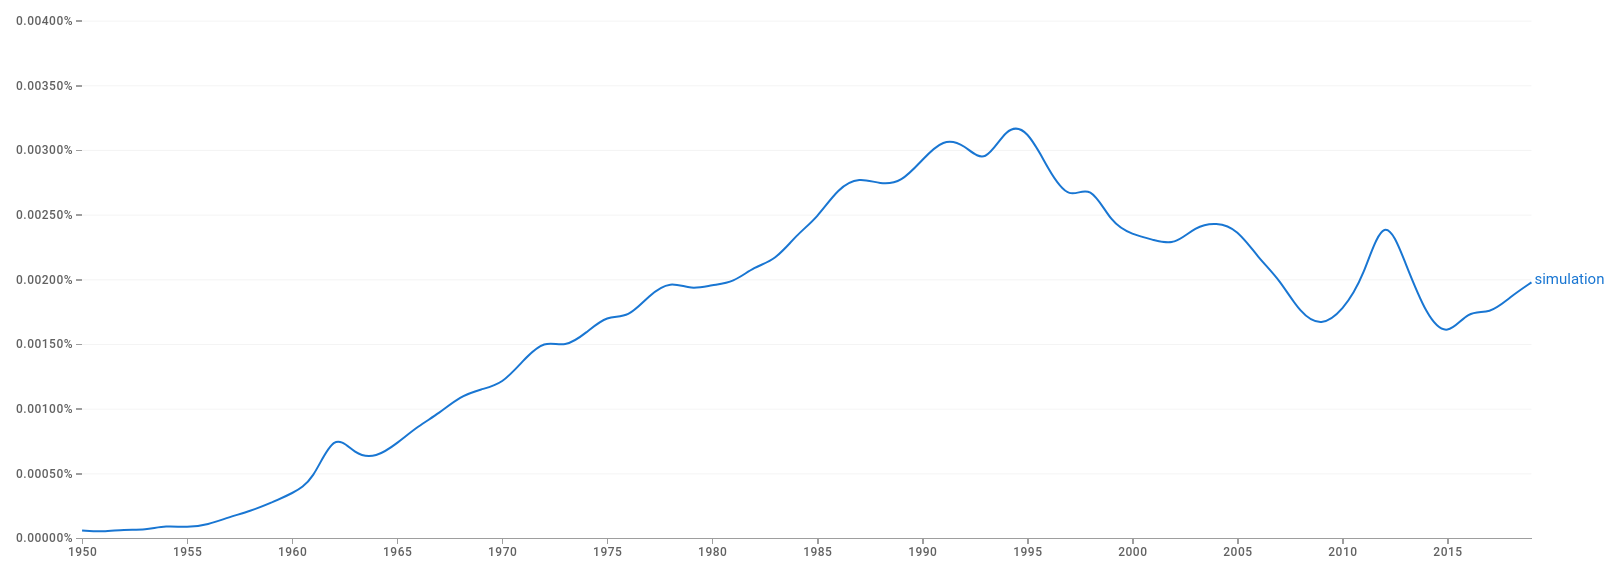
\includegraphics[width=0.7\linewidth]{Images/simulation_evolution_graph.png}
 	\caption{Evolution of the simulation topic in the literature by Google Books ngram viewer}
	 \label{fig_simulation_evolution_graph}
\end{figure}

Analyzing the market research report by ZION, is possible to conclude that the global virtual training and simulation market size was valued 
at \$332.6 Billion in 2022 and is projected to reach \$973.4 Billion by 2030.  

\begin{figure}[H]
	\centering
 	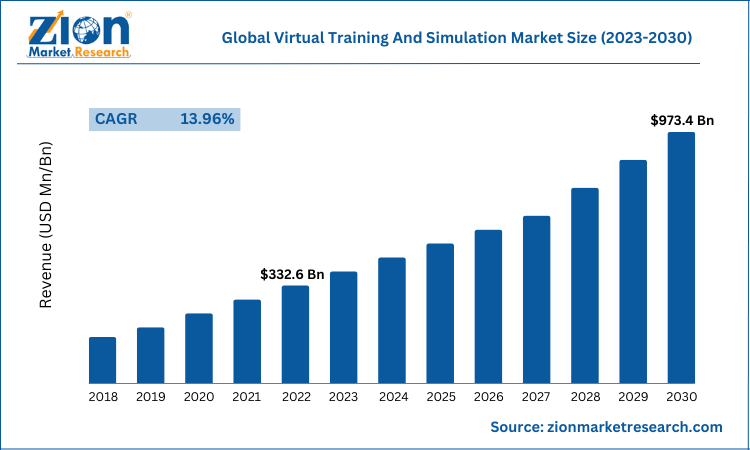
\includegraphics[width=0.7\linewidth]{Images/ZION_MarketResearch.png}
 	\caption{Market research report by ZION about simulation \cite{zionMarketResearch}}
	 \label{fig_ZION_MarketResearch}
\end{figure}

This growth and demand in the industry turn this topic into an important subject. For this reason, it is important to understand what is 
simulation and why is it necessary. In the following points, this will be covered in detail.

\subsection{Definition}
\label{subsec:WhatIsSimulation}

Accordingly the Cambridge dictionary, simulation can be defined as \emph{"a situation or event that seems real but is not real, used especially 
in order to help people deal with such situations or events"}. Moreover, simulation can be also defined, in a more general way, as 
\emph{"an imitation of a system"} \cite{SimulationBook}. Therefore, simulation is not exclusively confined to computers but also encompasses a 
diverse range of applications, whether physical or virtual. For instance, in the automotive industry, each new model that is designed must 
undergo a security test. One of the numerous examinations performed involves simulating a car crash into a wall and assessing the driver's 
resulting damages. As a result, conclusive determinations can be made, specifically in this case, regarding whether the car has successfully 
met the test's requirements or not.

Hence, simulation is a controlled verification technique that helps to understand how a system would behave in a real situation. As previously 
mentioned, simulation can be physical or virtual. Nowadays, the last is the preferable one, since it brings huge advantages when compared to the 
other. First of all, the cost. It is clear that physical simulations, like the one previously described, have a lot of associated costs. The car 
that is going to be destroyed, the workers to make sure everything goes as planned and to clear all the wreckage, and even the infrastructure, 
that require a designated area which involves costs and space. The second reason is the time. In a competitive industry, the first to have the 
product in the market can be the one that will have more success. Physical simulation can take a lot of time. It may be necessary, beyond the 
simulation itself, preparation, post-cleaning, license acquisition, weather conditions, etc. delaying the process. The last factor is the 
computer's evolution. As noted earlier, its evolution was crucial in the way that more complex simulation environments can be tested and obtain 
more accurate results.

To elaborate on the concept of virtual simulation, it can be classified into three categories. This classification is illustrated in 
the  \autoref{fig_VitualSimulation_ramification}, which outlines the taxonomy of virtual simulations. 

\begin{figure}[H]
	\centering
 	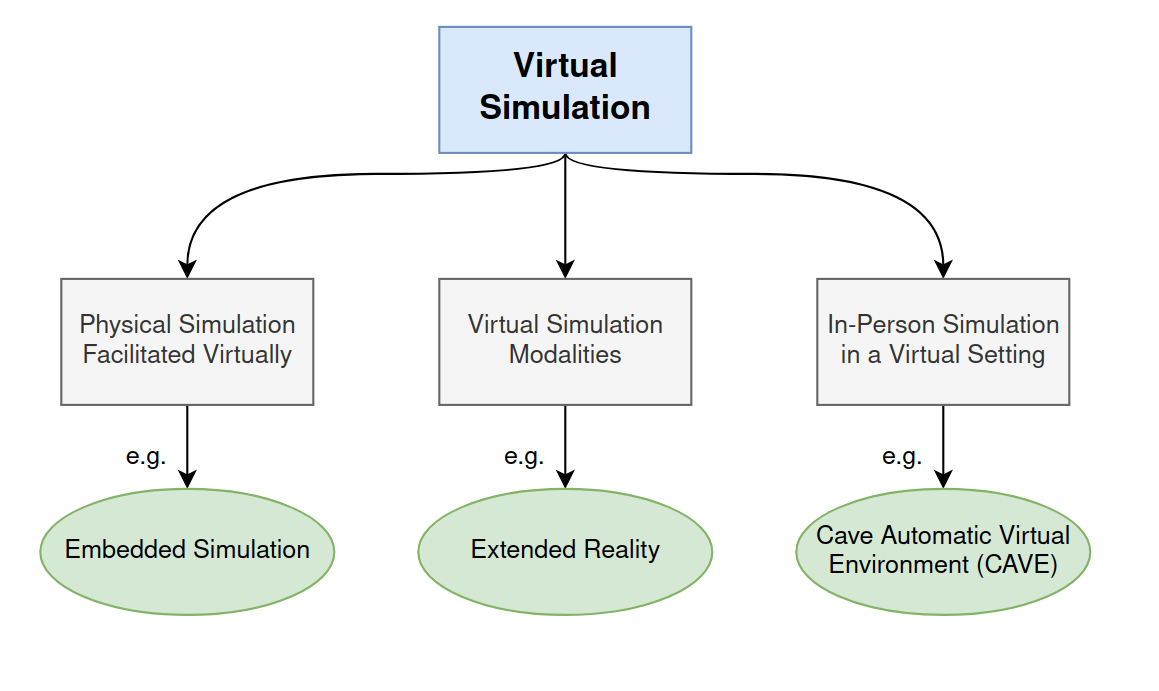
\includegraphics[width=0.7\linewidth]{Images/VitualSimulation_ramification.png}
 	\caption{Taxonomy of virtual simulations (Adapt from \cite{verkuyl2022virtual})}
	 \label{fig_VitualSimulation_ramification}
\end{figure}

 %https://ecampusontario.pressbooks.pub/vlsvstoolkit/chapter/technological-variety-in-virtual-simulation/

As shown, it can be divided into physical simulation facilitated virtually, virtual simulation modalities, and in-person simulation in a 
virtual setting. 

Physical simulation facilitated virtually is the process of utilizing virtual simulation to replicate a physical phenomenon or system. This 
is done through the creation of a digital model that imitates the physical object, and through various algorithms and computational methods, 
simulates its behavior in a virtual environment. In this way, it is possible to predict how the physical system will behave in various scenarios, 
without the need for physical testing, thereby saving time and resources. It is used, for example, in the development of an embedded system. 
Without it, it would be mandatory to have the physical prototype to evaluate if the system matches all the requirements. 

This dissertation will focus on computer architecture simulation. Therefore, the concept of simulation can be redefined as \emph{"the imitation 
of the operation of a real-world process or system over time"} \cite{banks1999introduction}. The computer architecture itself becomes the system 
under study, and simulation enables the user to explore its capabilities and limitations in a simulated environment.

\subsection{Importance of Simulation}

To have a full scope of why simulation is important, three topics should be considered: how the nature of the system affects the simulation, and 
the advantages and disadvantages of this technique compared to other validation methods \cite{SimulationBook}.

The first topic exhibits three characteristics: variability, interconnections, and complexity. Consider the production of a \gls{cpu} chip as an 
example. The production process may have interconnections with other factors such as the chip manufacturers or the chip designers. These 
interconnections can make it difficult to predict the overall performance of the system, which in this example is the \gls{cpu} chip production, 
especially when variability is present. Furthermore, systems can be complex, and these complexities make it challenging to predict the performance 
of a system when changes are made or actions are taken. With simulation models, these problems can be solved in a way that they can explicitly 
represent the variability, interconnectedness, and complexity of a wanted system.

Keeping the example of \gls{cpu} chip development, the process goes through various stages and, in the end, it is crucial to test the product 
before mass production. Thus, a prototype is built so tests can be made. However, building a prototype takes time and money. In the majority of 
cases, the prototype can be improved, so the developers need to go through the process again. A new cycle begins, which means spending more time 
and money. Simulation can solve this problem in the way that development and testing can be done in parallel. In other words, while the developers 
are creating the chip, it can be tested in simulation, even without the physical prototype. Moreover, simulation is flexible, which means small 
changes can be done easily, is controlled, that is, it can control the experimental conditions in the way direct comparisons can be done, 
and is transparent, so there are no subjective results.

In terms of drawbacks, it is possible that the development team consists solely of individuals specialized in \gls{cpu} chip design. Therefore, 
the team would need to hire a new employee with expertise in simulation to fulfill the requirements. Furthermore, it requires powerful computers 
and a huge sufficient storage capacity, as simulation results can be in the order of dozens of gigabytes. The software to run the simulation and 
the creation of the model to test require investments. All these aspects represent an enormous investment for the company, where it will not get 
a direct profit. On top of that, simulations are not 100\% accurate, meaning that they can produce results that are not the correct ones.

Considering all the aspects, simulation brings a lot of benefits when compared to other techniques, such as experimentation in real life. 
Nonetheless, the downsides must be taken into account and concluded whether this solution fits the needs or not. Banks in 
\cite{BanksDiscreteSimulation} mentions examples of applications where it can be used, like computer system performance, food processing, 
transportation systems, and embedded systems.


\section{Embedded Systems}

Embedded systems have a ubiquitous presence in modern life, from cars, computers, and televisions to smartphones and even toothbrushes. It is 
so common and present everywhere that the world without it wouldn't be the same. While this topic is not new to academia, with books like 
\cite{banks1999introduction} mentioning it as early as the 19th century, it has gained more attention and deeper analysis since the 1980s until 
nowadays. 

The following topics explain more about how can embedded systems be defined, and which are the development processes used in the industry. 
In the end, a specific topic about simulation in embedded systems will be covered.

\subsection{Definition}

The definition of embedded systems is not straightforward, that is, there is no agreement in the literature mostly because this term is being 
under development every day. One possible definition can be a combination of computer hardware and software, and perhaps additional mechanical 
or other parts, designed to perform a dedicated function \cite{EmbeddedSystemsGlossary}. Other authors prefer to highlight their relevant 
properties, like Raul Camposano in \cite{camposano1996embedded}, where he focuses on correctness, real-time, and dedicated functions, among 
others, as the important aspects to retain when an embedded system is mentioned. 

\begin{figure}[H]
	\centering
 	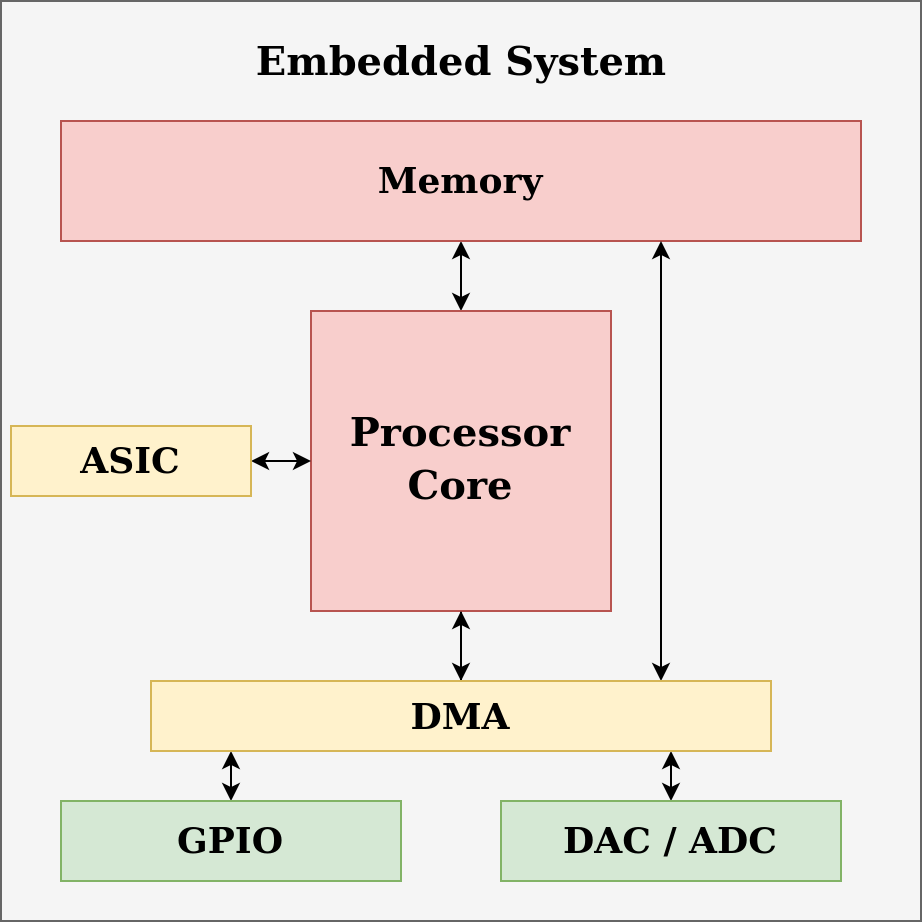
\includegraphics[width=0.6\linewidth]{Images/TypicalEmbeddedSystem.png}
 	\caption{Typical embedded system (adapted from \cite{camposano1996embedded})}
	 \label{fig_TypicalEmbeddedSystem}
\end{figure}

In the same work, he defined how a typical embedded system is, which is shown in the \autoref{fig_TypicalEmbeddedSystem}. The colors depicted 
in the figure indicate the significance of each component in the embedded system. Red denotes an indispensable part that must be present. Yellow 
means that it is not mandatory, although it is recommended. Green stands for optional, as it can be used or not depending on the application. The 
arrows are used to demonstrate if the communications between the different parts are one-directional or bidirectional. 

The processor core and memory are the two crucial components in an embedded system, as they are interdependent and cannot function without each 
other. Specifically, the processor requires the memory to access the data that needs to be processed, while the memory itself cannot perform any 
processing on its own. Therefore, the existence of both components is essential for the development of a functional embedded system. The \gls{dma} 
is a very important part of an embedded system. It is a hardware mechanism that allows peripheral components to transfer their \gls{io} data 
directly to and from main memory without the need to involve the system processor. Thus, the significance of this lies in its ability to avoid 
a substantial processor overhead \cite{LinuxDeviceDrivers}. \gls{asic}, as the name suggests, is used for specific applications where 
dedicated hardware is required. It can reduce significantly the execution time of certain applications \cite{FPGAaccelaration3} 
\cite{FPGAaccelaration2} \cite{FPGAaccelaration}. For this reason, many systems require dedicated hardware however, it will become a smaller 
fraction as time passes \cite{camposano1996embedded}. \gls{gpio}, \gls{adc}, and \gls{dac} are examples of parts that establish an interface 
between the embedded system and the external world, and so they can be needed or not depending on the requirements.

The range of embedded systems is very wide. It starts from low power, like receiving data from \gls{adc} and sending it to a database, to 
multi-core applications, for example, laptops, smartphones, or even tables. Hence, when designing a system, it is important to comply with 
the \gls{swapc} constraints, which means that the system can only use the essential resources, commonly referred to as "resource-constrained 
devices" \cite{swapc}. 

Furthermore, embedded systems should be dependable, that is, they should perform as and when required \cite{iec}. The following characteristics 
must be fulfilled for dependability, nevertheless, different applications can attend better to different topics. In the case of cars, trains, 
or planes, the focus should be more on safety, whereas databases or banks should prioritize security.

\begin{enumerate}
    \item \textbf{Reliability:} Continuity of service delivery while in use, e.g., the probability of the system working properly since it 
	worked after startup

    \item \textbf{Maintainability:} Capability to be retained in, or restored to a state to perform as required, under given conditions of 
	use and maintenance

    \item \textbf{Safety:} Ability to not cause catastrophic effects on the environment as a consequence of a 
	failure

    \item \textbf{Availability:} Capacity to be in a state to perform as required 
    
    \item \textbf{Security:} Capability to provide communication confidentiality and authentication
    
\end{enumerate}


\subsection{Operating Systems}

An embedded system can be complex. Take a laptop as an example. There are lots of different resources to manage, each one with its 
characteristics. Screen, mouse, keyboard, \gls{io} devices, and network interfaces are some examples. Creating code to control all of them 
efficiently is almost impossible since the programmer needs to understand in detail every component. \glsxtrfullpl{os} came to solve this 
problem by providing a software layer that not only abstracts all the details for the user but can also optimally manage all the resources. 
The next picture presents how an embedded system with a \gls{os} can be divided. It is important to point out that every embedded system does 
not need to have an \gls{os}, for example, a device that only reads a \gls{adc} port and sends the information does not need that. 

\begin{figure}[H]
	\centering
 	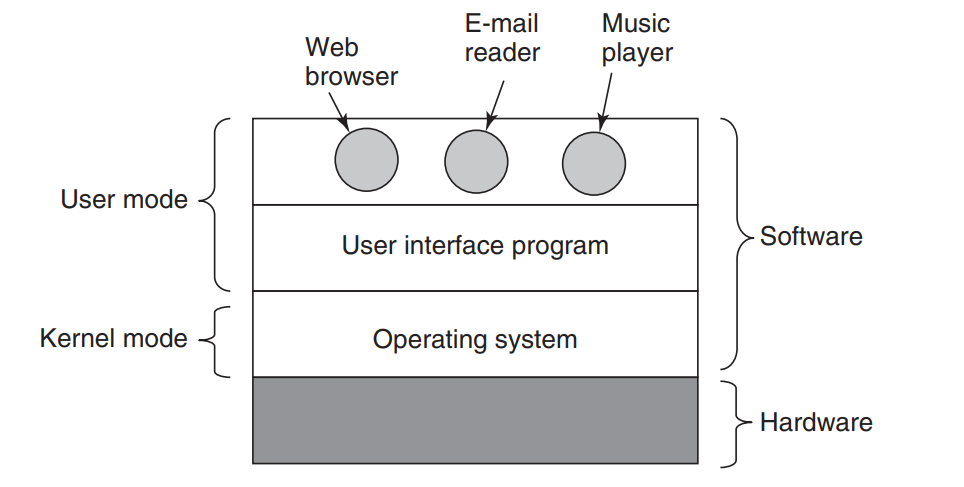
\includegraphics[width=0.6\linewidth]{Images/OS_overview.png}
 	\caption{Layers of an \gls{os} \cite{OSbook} }
	 \label{fig_OSoverview}
\end{figure}

% The hardware is mandatory in every embedded system because there's no software without hardware. Hardware refers to the physical components 
% of a system, such as a screen, mouse, memory, and board, among others. It encompasses all the tangible elements that make up a computer or 
% electronic device.

% The software layer can be divided into two sub-layers: kernel mode and user mode. The \gls{os} runs in the kernel mode and here the \gls{os} 
% has full control of the hardware, that is, it can execute any available instruction at any time. There are different operating systems in the 
% market and they can be open source (e.g. Linux) or paid (e.g. Windows). On top of that, there is the user mode, which is responsible for 
% providing an interface between the machine and the user. Now, some instructions cannot be executed directly, since it could affect the system's 
% well-behavior. There are two types of user interface programs: the text-based shell and the \gls{gui}, which is icon-based. With both 
% methods is possible to start up programs like the web browser, the music player, and so on.

Going into detail in the \glspl{os}, one important concept to keep in mind is the \textbf{process}, which is an instance of an executing 
program. Processes are crucial in a way that they allow the system to have multiple jobs at the same time. Following the previous example, a 
user with a laptop can play music and surf the internet at the same time. Even with one \gls{cpu}, \glspl{os} have the capability of keeping 
track of multiple processes, by switching from process to process speedily, creating the illusion of parallelism. This concept is called 
\textbf{concurrency} and it is illustrated in the \autoref{fig_ConcorrencyProcess}

\begin{figure}[H]
	\centering
 	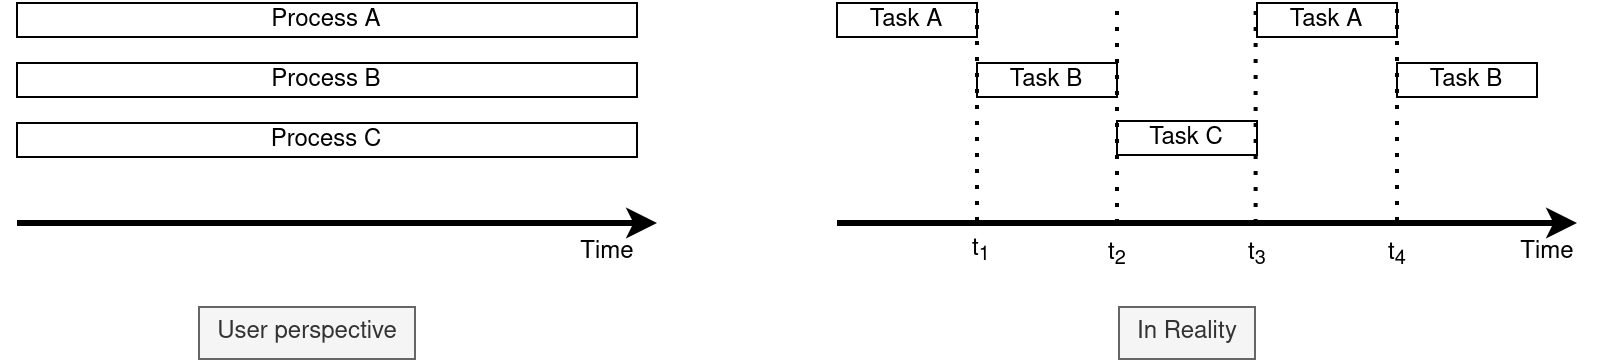
\includegraphics[width=1\linewidth]{Images/ConcorrencyProcess.png}
 	\caption{ Concurrency between processes }
	 \label{fig_ConcorrencyProcess}
\end{figure}

Note that, in this example, it is considered a system with one \gls{cpu} core. It is clear that if the system has more cores, which is common 
nowadays, the \gls{os} can split the work among them and have real parallelism. If the system has four \gls{cpu} cores, each core can execute a 
process at a time, increasing the performance even more. To do this concurrency, the \gls{os}, more precisely the \textbf{scheduler}, manages the 
processes by attributing states to them. There are three states: running (the process is in execution at that time), ready (the process is not 
running at the moment but it is ready), and blocked (the process is unable to run until some external event happens). 

When thinking about programs, it is clear that one can have multiple works to do at the same time, for instance, a web browser. It needs to 
display the content, receive the keyboard and mouse information, receive web packages, and so on. If it was only receiving the keyboard 
information, it wouldn't do the remaining jobs making the process inefficient. Therefore, processes can have multiple \textbf{tasks} that run 
within the process, which are called \textbf{threads}. Threads are essential for the following reasons \cite{OSbook}.

\begin{enumerate}
    \item They have the ability for the parallel entities to share address space and all of its data among themselves

    \item They are lightweight and easier/faster to create and destroy than processes (Around 10-100 times faster)

    \item They can increase performance when there is substantial computing and \gls{io} because it allows these activities to overlap

    \item They are useful on systems with multiple \glspl{cpu}, where real parallelism is possible
\end{enumerate}

Processes are assigned independent memory regions, and the threads within the process share the process memory between them. A process can 
have multiple threads, but a thread can have only one process associated. Without threads, a process contains one single stack and a set of 
registers. With threads, each of them has a stack and a set of registers. \textbf{Execution context} is represented with a combination of 
registers and stack, representing the \gls{cpu} state for each task. \autoref{fig_ProcessAndThread} illustrates the previous notion. 

\begin{figure}[H]
	\centering
 	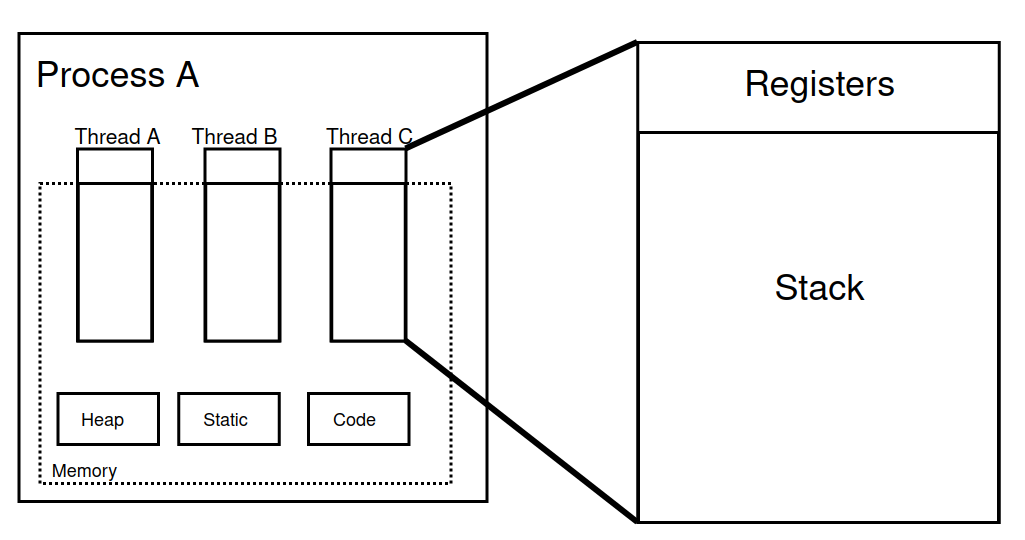
\includegraphics[width=0.7\linewidth]{Images/ProcessAndThread.png}
 	\caption{ Process and threads block diagram }
	 \label{fig_ProcessAndThread}
\end{figure}

With threads can also be applied concurrency, in order to have parallelism and better computational performance. As processes, the scheduler 
defines which task will be executed. There are four states: run (the task is in execution at that time), ready (the task is not running at the 
moment but it is ready), wait (the task is waiting for data), and null (the task is created or killed). \autoref{fig_ConcorrencyProcess} can also 
be applied to this context.

Nevertheless, in reality, when a task is running and another replaces it, there are some steps to pursue. First of all, it 
is necessary to save the \gls{cpu} state of the running task. After that, the scheduler needs to select another to get running. Then, it restores 
the context of the selected one, so it can transfer the execution control. All this process is called \textbf{\gls{cs}}. The time consumption of 
the \glspl{cs} are a problem, as present in the figure below. However, the benefits of having concurrency, as explained earlier in this section, 
are massive, and thus the trade-off is positive.

\begin{figure}[H]
	\centering
 	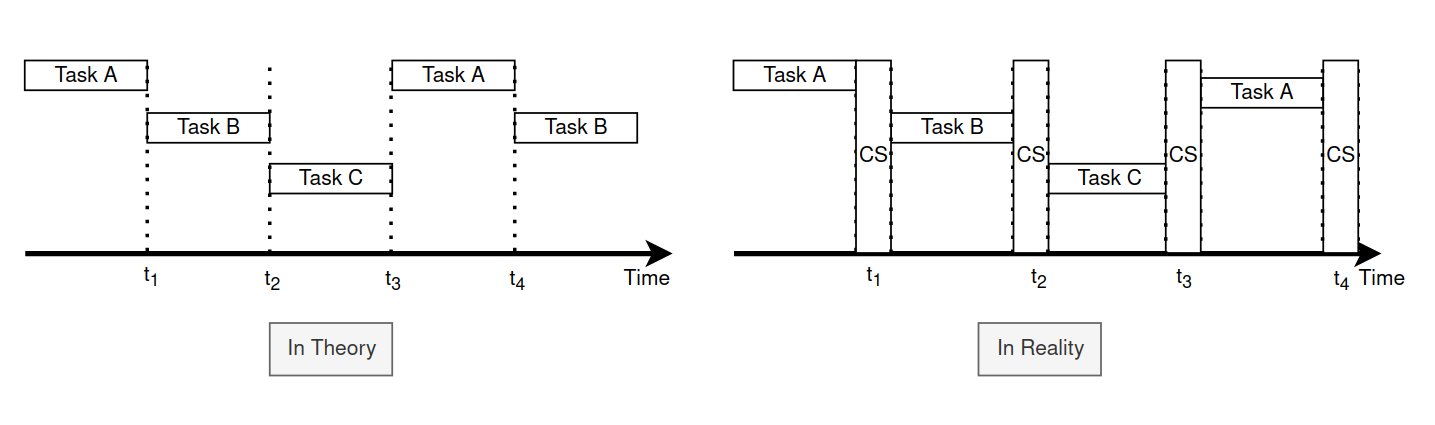
\includegraphics[width=1\linewidth]{Images/ContextSwitch.png}
 	\caption{ Context switch }
	 \label{fig_ContextSwitch}
\end{figure}

Another issue that can take plan is when two different processes are using the same memory. By definition, they are assigned independent 
memory regions, but there are situations where this is not true. The most common is when two or more different processes interact with each other, 
where one, for example, writes in the memory and the others read from it. To control this \textbf{\gls{ipc}}, two mechanisms were created: data 
transfer and shared data.

Data transfer involves the concepts of writing and reading. The most typical \glspl{ipc} are pipes and message queues. The main difference 
between both is pipes are uni-directional communication channels, while message queues are bidirectional.

Shared data is a memory region that is shared by multiple processes. Thus, if a process wants to share some data, it only needs to make it 
available in the shared memory region. For this reason, it is the fastest \gls{ipc} available because the data transfer occurs at the speed of 
memory access, but it is dangerous because it has the same meaning as global variables, so there is no control to access those. The next figure 
shows a possible problem that can happen with shared memory.

\begin{figure}[H]
	\centering
 	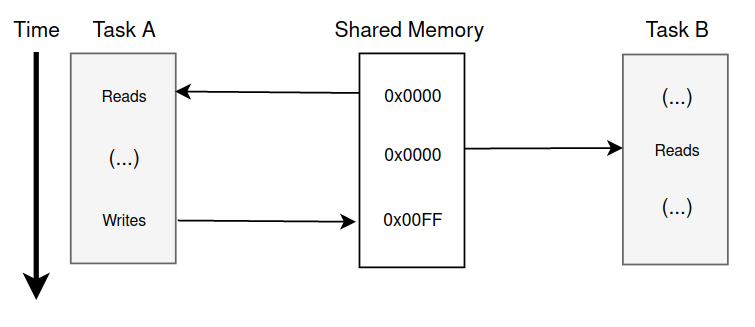
\includegraphics[width=0.7\linewidth]{Images/BeforeMutex.png}
 	\caption{ Two different tasks using the same resource }
	 \label{fig_BeforeMutex}
\end{figure}

In this example, task A reads the value from the shared memory region, executes an equation, and writes the result in the same variable. For 
instance, this equation can be as simple as summing 0xFF ( Y = X + 0xFF ). Task B reads that value and prints it on the terminal. As demonstrated 
in the figure, task B will read 0x0000 even though task A was using the variable. In the case of multiple tasks and the result of one matters to 
another, this issue can be a serious problem. This problem is called \textbf{race conditions}, and it is more critical with the increasing 
parallelism due to increasing numbers of cores.

To avoid that were created \textbf{task synchronization objects}. The most important methods are semaphores and mutexes. The first one can be 
divided into binary semaphores and counter semaphores, and they are useful methods to synchronize interrupts with a given task. The second one is 
a shared variable that can be in one of two states: owned or free. Binary semaphores and mutexes share many characteristics. Both can be utilized 
for mutual exclusion, ensuring that only one thread accesses a shared resource at a time, but only the first can be used for synchronization 
\cite{OSbook2}. Regarding the previous example, \autoref{fig_AfterMutex} illustrates the same situation but using a mutex.

\begin{figure}[H]
	\centering
 	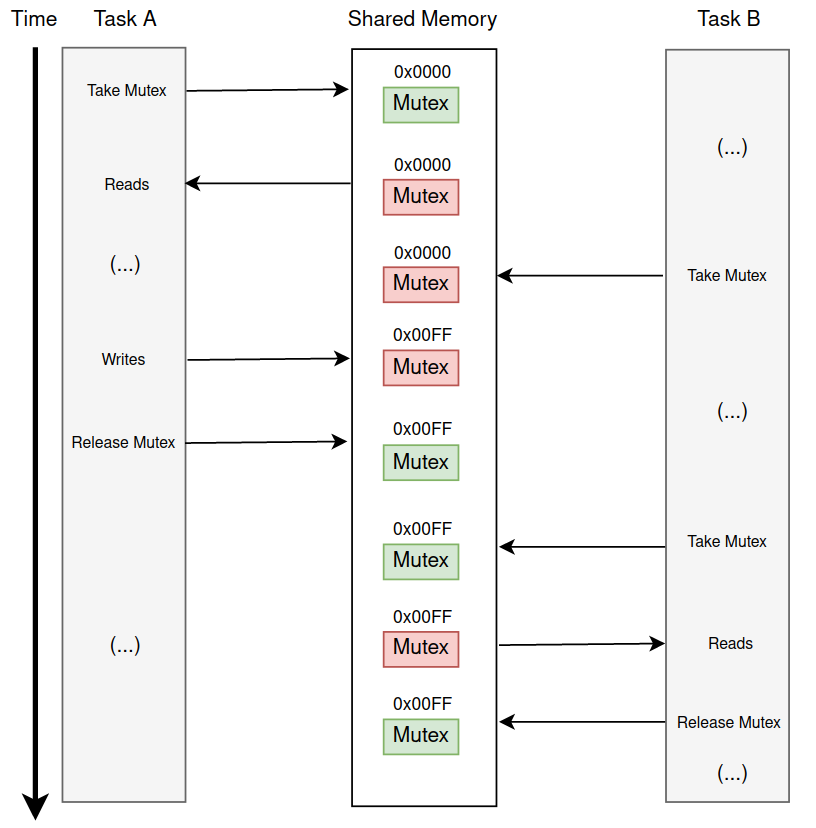
\includegraphics[width=0.7\linewidth]{Images/AfterMutex.png}
 	\caption{ Two different tasks using the same resource with mutex }
	 \label{fig_AfterMutex}
\end{figure}

Now, both tasks, before using the shared variable, need to take the mutex. If the mutex was already taken (first trial of task B), 
the task will receive a blocked resource response, meaning it is unavailable until the owner releases the mutex. 


\subsection{Development Models}
\label{sub_sec::DevModels}

When building an embedded system, several aspects should be taken into account, like its requirements, constraints, and levels of complexity, 
therefore one development model that works well for one project may not work well for another with different requirements or constraints. This 
section will present some examples of models typically used in the industry and research teams. There are a lot more models with different 
characteristics, thus before the beginning of the project, all possibilities must be considered.
\newline

\textbf{Waterfall model}
\newline

The traditional waterfall model is linear, that is, there are well-defined stages and once the project moves to the next stage, it can not go 
back \cite{waterfallModel}. \autoref{fig_Waterfall} represents the different stages of the model. 

\begin{figure}[H]
	\centering
 	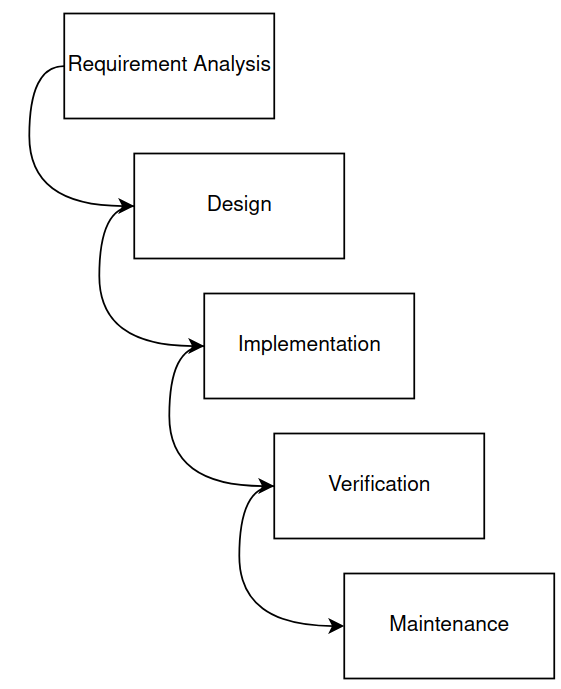
\includegraphics[width=0.4\linewidth]{Images/Waterfall.png}
 	\caption{The waterfall model}
	 \label{fig_Waterfall}
\end{figure}

Because of this linearity, no previous stages can be reviewed or improved, which makes the traditional waterfall model a good option for projects 
that have well-defined requirements and a short development cycle. Adetokunbo in \cite{waterfallModel} goes further and states that it is also 
viable to use it when altering the software after coding is very much prohibited.

Some variations allow for an iterative relationship between phases and even add more phases. Royce in \cite{royce1970winston} presents and 
explains some of them in detail. 
\newline

\textbf{V-Model}
\newline

The verification and validation model, more known as V-model, is a modified version of the Waterfall method \cite{V-model}. It is non-linear, 
which means that allows step-backs in the development process. An important aspect of this model is that testing activities like planning, and 
test designing happen well before coding, preventing bugs or bad-functional systems. \cite{V-model2}. The following picture shows a typical 
representation of this model.

\begin{figure}[H]
	\centering
 	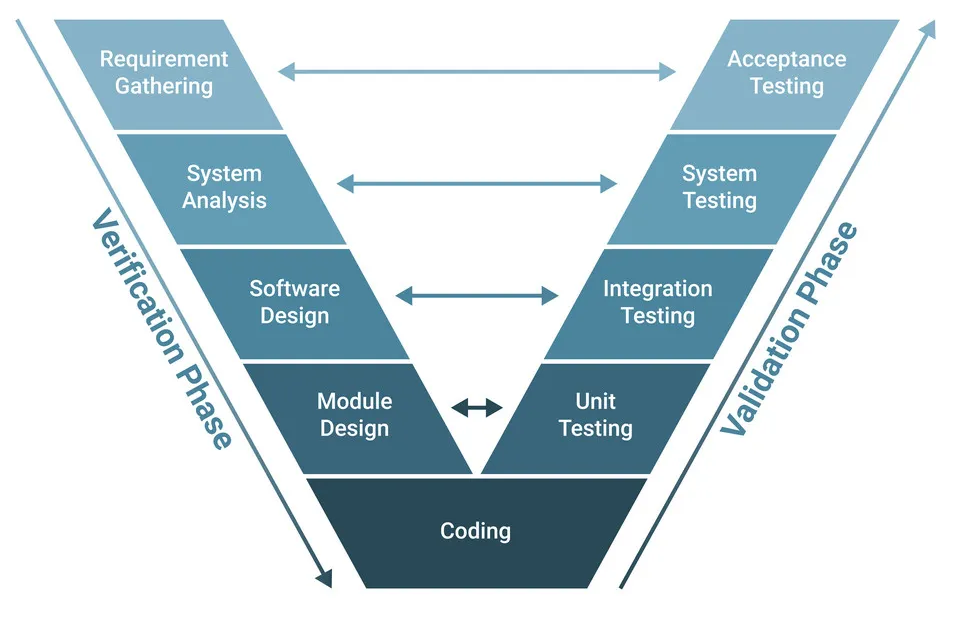
\includegraphics[width=0.5\linewidth]{Images/V-Model.png}
 	\caption{The V-Model}
	 \label{fig_V-Model}
\end{figure}

The main advantages are the proactive tracking of defects in the various phases, cost reduction in the correction of defects since these are 
spotted much sooner, and it is simple to understand and apply. On the other hand, it lacks flexibility as any changes require updating the majority 
of documents, demanding significant time and resources, which can make it challenging for companies to adopt. \cite{V-model} \cite{V-model2}. 
Nevertheless, it is arguably the most traditional model utilized for software test management. \cite{mathur2010advancements}.

Other variations try to improve these downsides. Some examples are the shark tooth and W-model \cite{V-model2}.
\newline

\textbf{Agile Model}
\newline

Although there are lots of agile techniques, they share common characteristics, including iterative development and a focus on interaction, 
communication, and the reduction of resource-intensive intermediate artifacts \cite{waterfallAndAgile}. Therefore, this model states that the 
project should be divided into mini-projects to remove unnecessary activities that waste time and effort. These mini-projects have requirements 
analysis, design, implementation, and test \cite{waterfallAndAgile}, and should not exceed 30 days \cite{AgileModel}. In the end, all are 
combined to obtain the final project.

\begin{figure}[H]
	\centering
 	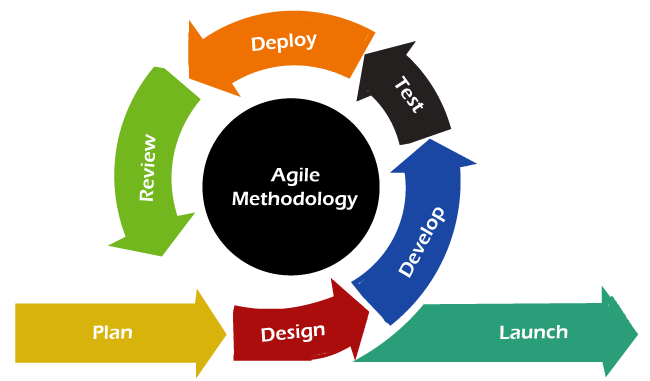
\includegraphics[width=0.5\linewidth]{Images/agileModel.png}
 	\caption{The agile model}
	 \label{fig_Agile}
\end{figure}

\autoref{fig_Agile} shows the agile model. In the review stage, an important aspect happens, which is customer interaction. 
The customer adaptively specifies his requirements for the next release based on the observation of the current release, rather than speculating 
at the start of the project \cite{SpiralModel}. 
\newline

\textbf{Spiral Model}
\newline

The spiral model is similar to the agile model, nevertheless, this one focuses on risk assessment and minimizing project risk. This can be 
achieved by breaking a project into smaller segments, which then provide more ease of change during the development process \cite{SpiralModel2}. 
In \autoref{fig_SpiralModel} is presented the spiral model. It is possible to notice that it requires a lot of time spent to evaluate the risks 
and planning or reevaluating the project every time a cycle is complete.

\begin{figure}[H]
	\centering
 	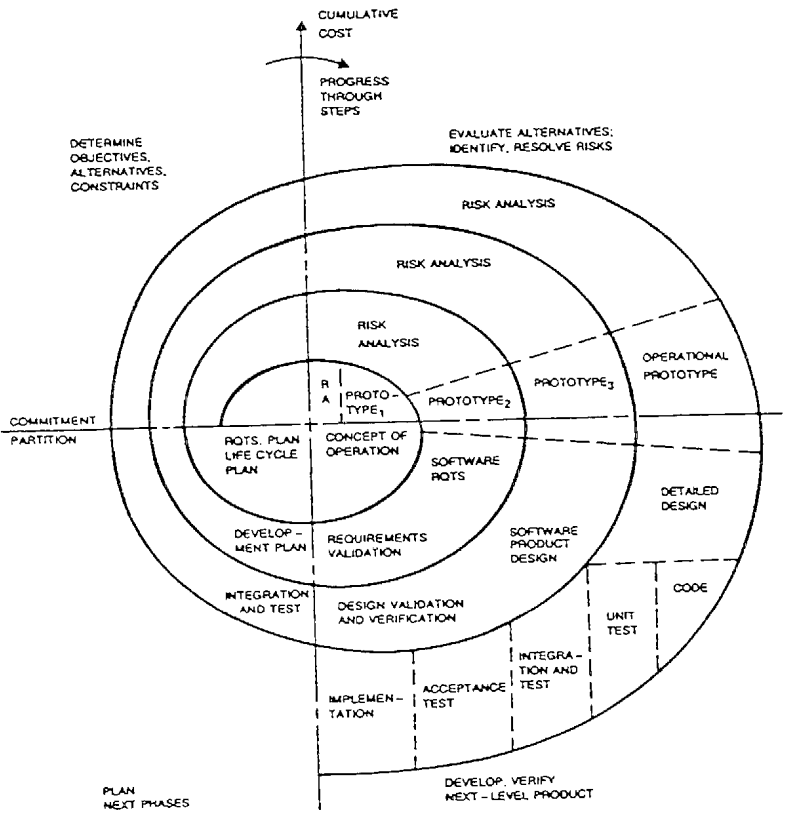
\includegraphics[width=0.5\linewidth]{Images/SpiralModel.png}
 	\caption{The spiral model \cite{SpiralModel3}}
	 \label{fig_SpiralModel}
\end{figure}

Hence, this model is recommended for medium to high-risk projects, when risk evaluation 
and costs are important, and when significant changes are expected \cite{SpiralModel2}. Moreover, it is also applicable to very large, complex, 
and ambitious projects \cite{SpiralModel3}


\subsection{Embedded Simulation}
\label{subSec::EmbeddedSim}

All the models presented in the \autoref{sub_sec::DevModels} have the verification stage, which is crucial to validate if the developed system 
meets the desired specifications. This validation normally requires the construction of a prototype in a way that engineers can evaluate its 
performance, test its functionality, and identify any potential issues or shortcomings. For example, in the automotive industry, where the most 
commonly adopted model is the V-model \cite{liu2016incremental}, the construction of a mock-up is necessary to identify flaws, delaying the 
overall development process. 

Therefore, simulation in the context of embedded systems is essential since the system can be tested without having the physical prototype, and 
some requirements, such as cache hits/misses, and computer performance, can be evaluated \cite{pargem5}. A simulator of this type is commonly 
referred to as a \acrfull{fss} or a \acrfull{vp}, and they can be described as a computer architecture simulator that simulates software in an 
electronic system, being this independent of the nature of the host computer. Usually, this term is mixed with emulation because although it 
can also run software tests inside flexible, software-defined environments, an emulator goes beyond by simulating both software and hardware 
configurations, being useful to test how software interacts with underlying hardware or a combination of hardware and software.

There are two types of \glspl{fss}, full system hardware simulator and full system software simulator. The hardware version offers a 
cycle-accurate simulation. As the name suggests, this technique is employed to perform a comprehensive analysis of the simulated embedded system 
at the clock level. Therefore, it is possible to accurately simulate hardware state transitions, obtaining specific information as the state of 
all logic gates or registers. Nevertheless, it can have very poor simulation performance because hardware-level simulators are not suited for 
the simulation of such complex systems as the embedded ones \cite{TypesOfFSS}. \autoref{fig_FSShardware} shows the simulation of a system using 
a hardware simulator. Some examples of this kind of simulator are GHDL \cite{GHDLMainHomePage} and Icarus Verilog \cite{williams2002icarus}.

\begin{figure}[H]
	\centering
 	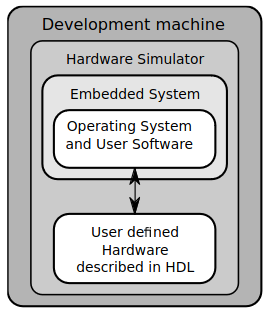
\includegraphics[width=0.3\linewidth]{Images/FSShardware.png}
 	\caption{Full system hardware simulator \cite{TypesOfFSS}}
	 \label{fig_FSShardware}
\end{figure}

The software version typically employs instruction-accurate simulation, where computations are performed according to the instruction set. 
However, this type of simulation does not provide information about the execution time of each instruction, resulting in a less detailed simulation 
that runs faster. Because of that, the hardware is not described in \gls{hdl}, unlike the previous version, as presented in the 
\autoref{fig_FSSsoftware}.

\begin{figure}[H]
	\centering
 	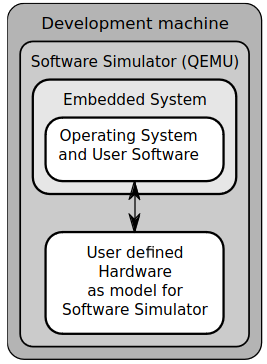
\includegraphics[width=0.3\linewidth]{Images/FSSsoftware.png}
 	\caption{Full system software simulator \cite{TypesOfFSS}}
	 \label{fig_FSSsoftware}
\end{figure}

The hardware model must be defined for the software simulation, thus these may or may not be available for the target machine. It 
requires the selection of a simulator that aligns with the application scenario or offers the flexibility to expand the range of supported hardware 
modules, such as QEMU \cite{theQEMUsimulator} and Gem5 \cite{TheGem5Simulator}.

As modern embedded and integrated systems become increasingly complex, an escalating number of design companies are embracing virtual prototyping 
methods \cite{UltraFastVPs}. \Glspl{vp} should follow this trend, that is, as embedded systems are becoming more complex, \glspl{vp} should be 
faster yet accurate, so they can be a reliable option.

The problem is \glspl{vp} are not following this evolution, which results in low performance, and thus high simulation times \cite{pargem5} 
\cite{UltraFastVPs} \cite{optimizingTD}. Although several works try to solve the problem, none of them have been able to 
provide an effective solution.

 

\section{Discrete Event Simulation}

% The definition of discrete-event simulation can be given as a technique used to simulate the operation of a system by modeling it as a sequence of events that occur over time. Exploiting this definition more in detail, there are concepts that should be define

%  An event is an instantaneous occurrence that changes the state of the system. Each event occurs at a particular instant in time and marks a change of state in the system.  

% In simulation, an event is a point in time when a the state of the system changes. \cite{SimulationBook}

Simulations, while valuable, cannot guarantee 100\% reliability due to certain scenarios that may be challenging to evaluate. For instance, 
certain physical phenomenon modeling may not be fully accurate when compared with real-world behavior. However, to enhance reliability, an 
simulator should strive to accurately represent real-world conditions. \gls{des} aligns with these requirements by simulating system dynamics 
event by event and providing comprehensive performance reports.

A \gls{des} can be defined as a simulation technique where state changes (events) happen at discrete instances in time. Events take zero time 
to happen, and it is assumed that nothing happens between two consecutive events that is, no state change takes place in the system between the 
events. A group of events organized by execution order is called an event queue or process \cite{DESVarga} \cite{SimulationBook}. From this point 
forward, whenever the term "process" is mentioned, it specifically refers to the event queue.

Consider a supermarket as an illustrative example. A supermarket system consists of one employee and two cashiers, PAY1 and PAY2. In this context, 
three events can be specified, and they are related to each other as shown in the \autoref{fig_DESscheme}.

\begin{itemize}
    \item Customer arrives at the supermarket (CA)
    \item Customer goes to the cashier (PAY1 / PAY2)
    \item Customer leaves the supermarket (CL)
\end{itemize}

\begin{figure}[H]
	\centering
 	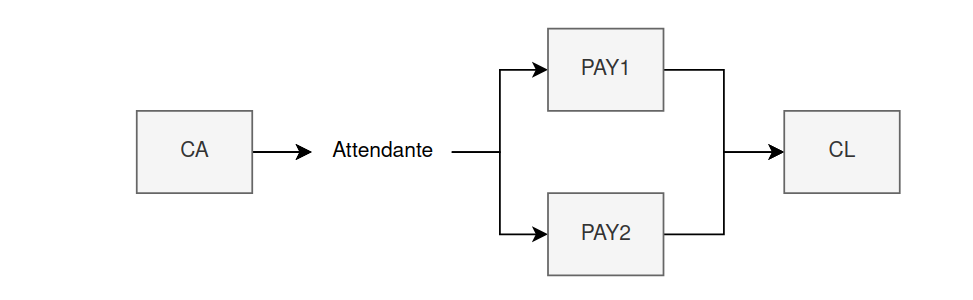
\includegraphics[width=0.9\linewidth]{Images/DES_Scheme.png}
 	\caption{Supermarket flow schematic}
	 \label{fig_DESscheme}
\end{figure}

Clients arrive randomly at the facility, and an attendant directs them to a cashier, according to the following rules: Whether both cashiers 
are available, the customer goes to PAY1; If only one of them is free, the client goes there; If both are occupied, the buyer waits until one is 
ready; If another buyer wants to pay, a queue is created following a \gls{fifo} style. The next table presents a situation assuming five clients 
and a payment time of five units of time. 

\begin{table}[H]
\centering
\begin{tabular}{llll}
\cline{1-3}
\multicolumn{1}{|l|}{\cellcolor[HTML]{9B9B9B}\textbf{Event number}} & \multicolumn{1}{l|}{\cellcolor[HTML]{9B9B9B}\textbf{Time}} & \multicolumn{1}{l|}{\cellcolor[HTML]{9B9B9B}\textbf{Event description}} &  \\ \cline{1-3}
\multicolumn{1}{|l|}{1} & \multicolumn{1}{l|}{1} & \multicolumn{1}{l|}{CA1} &  \\ \cline{1-3}
\multicolumn{1}{|l|}{2} & \multicolumn{1}{l|}{1} & \multicolumn{1}{l|}{CA1 goes to PAY1} &  \\ \cline{1-3}
\multicolumn{1}{|l|}{3} & \multicolumn{1}{l|}{3} & \multicolumn{1}{l|}{CA2} &  \\ \cline{1-3}
\multicolumn{1}{|l|}{4} & \multicolumn{1}{l|}{3} & \multicolumn{1}{l|}{CA2 goes to PAY2} &  \\ \cline{1-3}
\multicolumn{1}{|l|}{5} & \multicolumn{1}{l|}{4} & \multicolumn{1}{l|}{CA3} &  \\ \cline{1-3}
\multicolumn{1}{|l|}{6} & \multicolumn{1}{l|}{5} & \multicolumn{1}{l|}{CA4} &  \\ \cline{1-3}
\multicolumn{1}{|l|}{7} & \multicolumn{1}{l|}{6} & \multicolumn{1}{l|}{CL1} &  \\ \cline{1-3}
\multicolumn{1}{|l|}{8} & \multicolumn{1}{l|}{6} & \multicolumn{1}{l|}{CA3 goes to PAY1} &  \\ \cline{1-3}
\multicolumn{1}{|l|}{9} & \multicolumn{1}{l|}{7} & \multicolumn{1}{l|}{CA5} &  \\ \cline{1-3}
\multicolumn{1}{|l|}{10} & \multicolumn{1}{l|}{8} & \multicolumn{1}{l|}{CL2} &  \\ \cline{1-3}
\multicolumn{1}{|l|}{11} & \multicolumn{1}{l|}{8} & \multicolumn{1}{l|}{CA4 goes to PAY2} &  \\ \cline{1-3}
\multicolumn{1}{|l|}{12} & \multicolumn{1}{l|}{11} & \multicolumn{1}{l|}{CL3} &  \\ \cline{1-3}
\multicolumn{1}{|l|}{13} & \multicolumn{1}{l|}{11} & \multicolumn{1}{l|}{CA5 goes to PAY1} &  \\ \cline{1-3}
\multicolumn{1}{|l|}{14} & \multicolumn{1}{l|}{13} & \multicolumn{1}{l|}{CL4} &  \\ \cline{1-3}
\multicolumn{1}{|l|}{15} & \multicolumn{1}{l|}{16} & \multicolumn{1}{l|}{CL5} &  \\ \cline{1-3}
 &  &  & 
\end{tabular}
\caption{Example of a sequence of events in a supermarket}
\label{tab_DESexample}
\end{table}

When the time between arrival and reaching the attendant is considered to be zero, it indicates that there is no significant activity occurring. 
Otherwise, an additional event would have been included. In addition, when an event occurs, it is referred to as an event timestamp, typically 
measured in the same unit as the time within the model, known as the simulation time. Wall clock time or \gls{cpu} time refers to how long the 
simulation program has been running and how much \gls{cpu} time it has consumed on the target system. On the other hand, the amount of time 
spent, known as host or real-time, represents the actual duration taken to perform the simulation.

In this example, some events depend on others, for instance, event number eight is executed only when event seven has been executed as well. 
However, others are independent, like events one and two. So, even in this simple case, there are relationships between events that can complicate 
the concurrent execution of events, not allowing for a reduction in wall clock time.

This method has applications not only in the context of embedded systems but also in a wide area of topics. It is traditionally used for 
industrial applications, for example, in the design and evaluation of new
manufacturing processes, and in the establishment of optimum operational policies \cite{DES_SoA}. 

%Yet in the 1980s and 1990s, there was rapid development in this area, nowadays it does not verify, being the service sector the one that has 
% been expanding fast \cite{DES_SoA}. A comparison between these two sectors is imaginable in the way that both have different scenarios to take 
% into account and what-if questions. Some examples are: banking and finance services, healthcare and hospitals, and logistics and transportation 
% \cite{DES_SoA}. 
 
\subsection{Continuous Event Simulation}

Besides \gls{des}, there is another simulation technique, which is the \glsxtrfull{ces}. The perfect one does not exist, since they should be 
chosen to take into account the application, therefore a brief explanation will be made to understand when one is better than another.

Continuous simulation is used for modeling systems with continuous or analog behaviors. The state changes are continuous since they are modeled 
by differential equations. \cite{continousSim1} and \cite{continousSim2} are examples of applications where the authors decided to use this 
technique. 

\begin{figure}[H]
	\centering
 	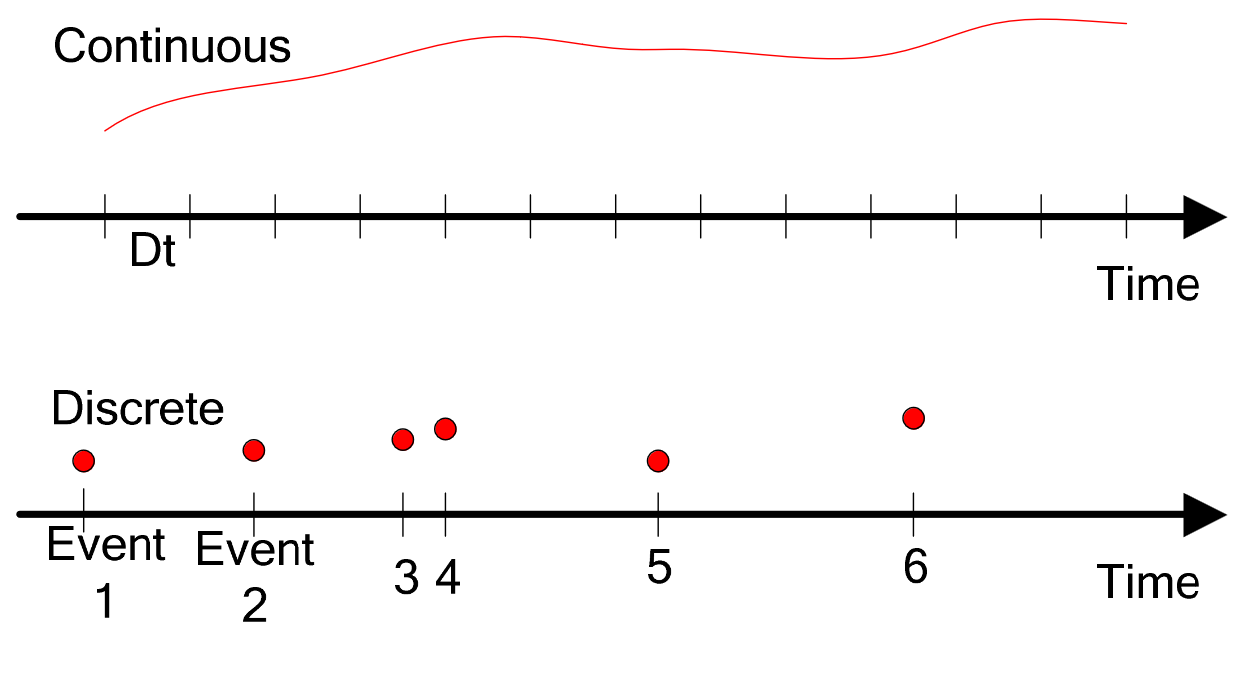
\includegraphics[width=0.7\linewidth]{Images/DesVsCes.png}
 	\caption{Updating state over simulated time in continuous and discrete simulation \cite{helal2008hybrid}}
	 \label{fig_DesVsCes}
\end{figure}


\section{Simulation Modes}

Different \glspl{fss} can use different modes to perform the simulation. These modes have an impact on the performance and accuracy of the 
simulation. For example, while Gem5 is limited to sequential simulation \cite{TheGem5Simulator}, QEMU offers the flexibility to be used in both 
sequential and parallel simulation \cite{QEMUDoc}. Depending on the application and the requirements of the project one option can be better 
than another.

According to \cite{parallelTypes}, there are two dominant approaches to advance time within a simulation, asynchronous and synchronous methods. 
In the first one, each thread communicates with the others in a way that each one can determine when it is secure to execute an event. The number 
of synchronizations can be reduced by far, although knowledge about the communication behavior of models and deadlock mechanisms, such as 
roll-back, is required. The second one uses global synchronization times to synchronize all threads. Between these times, all events that will 
be executed between them can be parallelized. This approach is simpler, nevertheless, it may incur high simulation overhead.

This section will present the two available modes, the sequential and the parallel. Nonetheless, it will also explain 
the \gls{td} technique, since both can use it in order to obtain more performance. Moreover, all further context will be related to 
the \gls{des} technique and the synchronous approach.

\subsection{Sequential Simulation}

Sequential simulation, or \gls{sdes}, is the most simple and accurate simulation mode. It executes the workload sequentially, that is, each event 
executes at its simulation time, resulting in a perfect simulation without any error. 

Going into detail, the simulator runs the process corresponding or sensitive to an event that should be executed at a specific timestamp. This 
process will run until a certain time when another event must be executed, and it is not related to the process in execution. In this 
exchange, there is a \gls{cs}, where happens a synchronization with the rest of the system. All variables are updated, thus, when a 
process reads or writes a variable, it accesses the state of the variable as it would be at the current simulation time. The coming image shows 
a sequential simulation with two different processes.

\begin{figure}[H]
	\centering
 	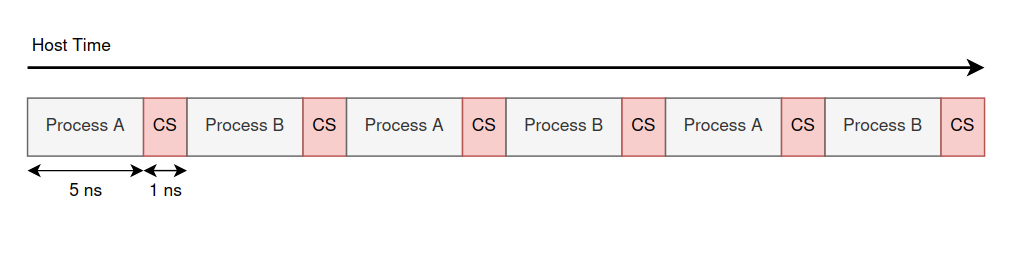
\includegraphics[width=0.8\linewidth]{Images/SequentialSimulation.png}
 	\caption{Example of a sequential simulation}
	 \label{fig_SequentialSimulation}
\end{figure}

Picture a scenario of a dual-core system with two processes where each event corresponds to an execution of an instruction with constant 
time (five nanoseconds), and each \gls{cs} takes one nanosecond. If the simulation lasts for one minute, ten seconds would be just for \glspl{cs}. 
It is visible that it spends a lot of simulation time, and it tends to get worse if more processes are needed. The overhead of the event 
scheduling and process context switching become the dominant factor in simulation speed, leading to a huge host time.

\subsection{Temporal Decoupling}

A technique used by SystemC, which is a standard C++ class
library for system and hardware design, to improve performance is \gls{td} \cite{systemC}. \gls{td} is a technique where individual 
processes are permitted to run ahead in a local time, without actually advancing simulation time, until they reach the point when they need to 
synchronize with the rest of the system. This time slice, from the beginning of the execution until the synchronization, is called 
\textbf{quantum}. The usage of \gls{td} may result in a faster simulation in some cases since it increases the data and code locality and 
reduces the scheduling overhead of the simulator. \autoref{fig_SequentialSimulationTD} shows the application of \gls{td} to the previous example. 

\begin{figure}[H]
	\centering
 	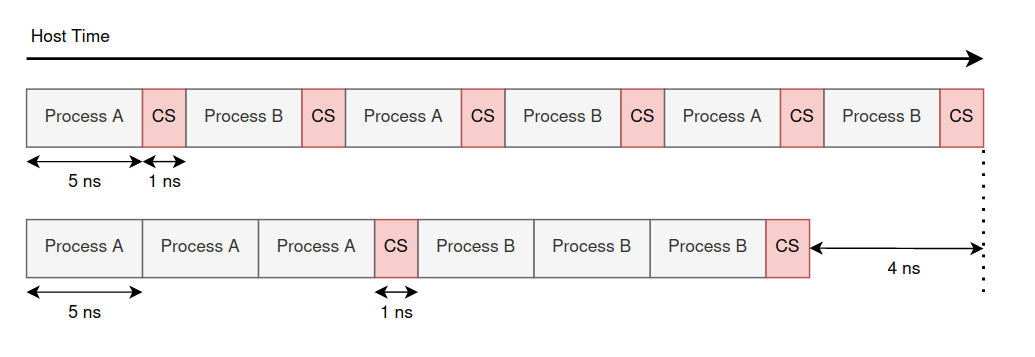
\includegraphics[width=0.8\linewidth]{Images/SequentialSimulationTD.png}
 	\caption{The principal of temporal decoupling}
	 \label{fig_SequentialSimulationTD}
\end{figure}

Now, for the same process execution time, the host time was smaller ensuring the existence of less \glspl{cs}. In this example, the reduction 
was four nanoseconds (four \glspl{cs}), circa 11\% of host time, compared to the approach without \gls{td}. It can be even higher if more 
processes and \glspl{cs} were being simulated.


As mentioned earlier, the process is permitted to advance beyond the current simulation time until it requires interaction with another process. 
This interaction could involve reading or updating a variable that belongs to another. At the moment, two things can happen: either access the 
current value and proceed, sacrificing accuracy or request synchronization and continue its process when the simulation time aligns with its 
local time. Proceeding with the current value entails making assumptions about communication and timing within the modeled system. It assumes 
there will be no adverse consequences when sampling or updating the value either too early or too late. Typically, this assumption holds in 
the context of a virtual platform simulation, where the software stack is designed to be independent of the underlying hardware 
timing intricacies.

Each process is responsible for evaluating whether it can progress beyond the current simulation time without compromising the functionality 
of the model. This is a SystemC characteristic because it guarantees functional congruency with the standard semantics of the simulator thus, 
it is not a mandatory feature to implement in other situations. 

Nevertheless, a problem can occur if the process does not respect the previous rule and runs with no restrictions. Other processes will not be 
able the run, compromising the system's functionality. A solution is to define a global quantum that forces the synchronizations. This global 
quantum, in the original version of SystemC, is static, which means it is defined by the user before the simulation and never changes. Forcing 
the synchronization results in another problem which is the trade-off between speed and accuracy. A small global quantum guarantees that the 
processes are using always the updated values and the simulator does not crash, therefore the accuracy will be high. However, the simulation 
speed will be sacrificed as more \glspl{cs} are occurring. On the opposite side, if the time slice is big, means that the system might introduce 
timing inconsistencies, which can lead, in the worst case, to a crash in the simulator. Hence, this value must be chosen carefully in order to 
have a fast yet accurate simulation.  

The SystemC reference manual \cite{systemC} enforces that some processes cannot be temporally decoupled due to their characteristics, thus 
they might become a simulation speed bottleneck. 

From here onwards, whenever the word "quantum" is mentioned, it refers to the global quantum.

\subsection{Parallel Simulation}

In the parallel mode, or in a \gls{pdes}, as the name suggests, the simulation uses more than one simulation thread in order to have real 
parallelism. In consequence, the host time will be smaller compared to the sequential mode, since multiple processes can be running at the 
same time. The next figure shows the speed difference between the two modes.

\begin{figure}[H]
	\centering
 	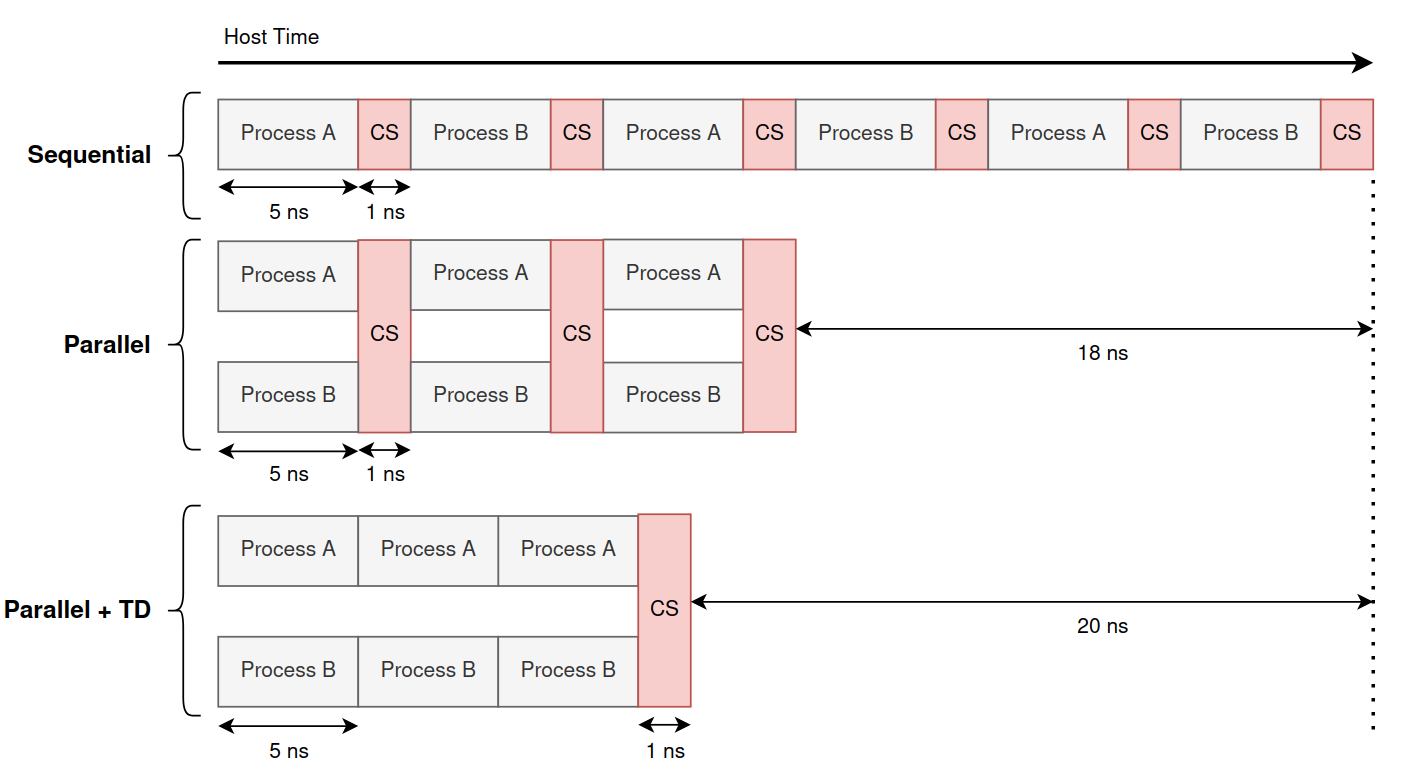
\includegraphics[width=1\linewidth]{Images/ParallelSimulation.png}
 	\caption{Sequential VS parallel simulation with and without \gls{td}}
	 \label{fig_ParallelSimulation}
\end{figure}

Continuing the previous scenario, with the parallel mode, the simulation can be fully optimized in a way that each process can have its 
execution thread. For this reason, the performance of the simulation increases a lot. In this case, for the same number of executed processes, 
the parallelized version was able to reduce eighteen nanoseconds of host time, which means a reduction of 50\%. With \gls{td}, the gain was 
pushed further when compared to the approach without it. However, it does not only offer advantages due to the 
several challenges that make achieving \gls{pdes} difficult. Typical problems are load imbalance, limited parallel work, and causality 
errors \cite{yoga2019parallelism} \cite{zhou1992sequential}. 

When working with tasks there is always the problem of balancing the workload among them to make an efficient use of today's multicore 
computers. An inefficient distribution can create performance bottlenecks. For instance, a system is programmed to read two different 
\gls{gpio} ports, do a logical XOR between both, and write in another \gls{gpio} port the result (to turn on a \gls{led}) and send it to 
the terminal. This workload results in four events, which will be assigned to two processes. If process A is attached with only one event, 
e.g. sending the information to the terminal, process B will be overloaded, and vice-versa. This issue is easy to solve in this simple 
example, but in programs with thousands \gls{loc}, it is a challenging job. \cite{loadImbalance1} and \cite{loadImbalance2} are examples of 
works that help to detect and measure the work imbalance.

It is rational to think that, after observing \autoref{fig_ParallelSimulation}, more parallelism will provide an even faster simulation, but 
this is not true. Normally programs can be parallelized until some point, like the previous example.
It is possible to simulate this system with four 
cores however, it is clear extra cores will not execute anything because there are no more processes to run. For this reason, 
the performance will not be improved, and the opposite can happen, that is, it becomes even worse \cite{scabilityIssue}. Some works identify 
this scalability problem to show the programmer how it can be improved \cite{scalabilityProblem} \cite{scalabilityProblem2}.

The last problem arises when there are causality errors. Causality errors happen when one event in the future affects an event in the past. 
Sequential simulation ensures that event B will execute after event A if the timestamp of event A is smaller than the timestamp of event B. 
In this mode that cannot happen, and if event B tries to change the state variables used by event A, a causality error happens. The following image 
illustrates the previous scenario, with events colored in green denoting "in execution," and events in gray indicating "scheduled".

\begin{figure}[H]
	\centering
 	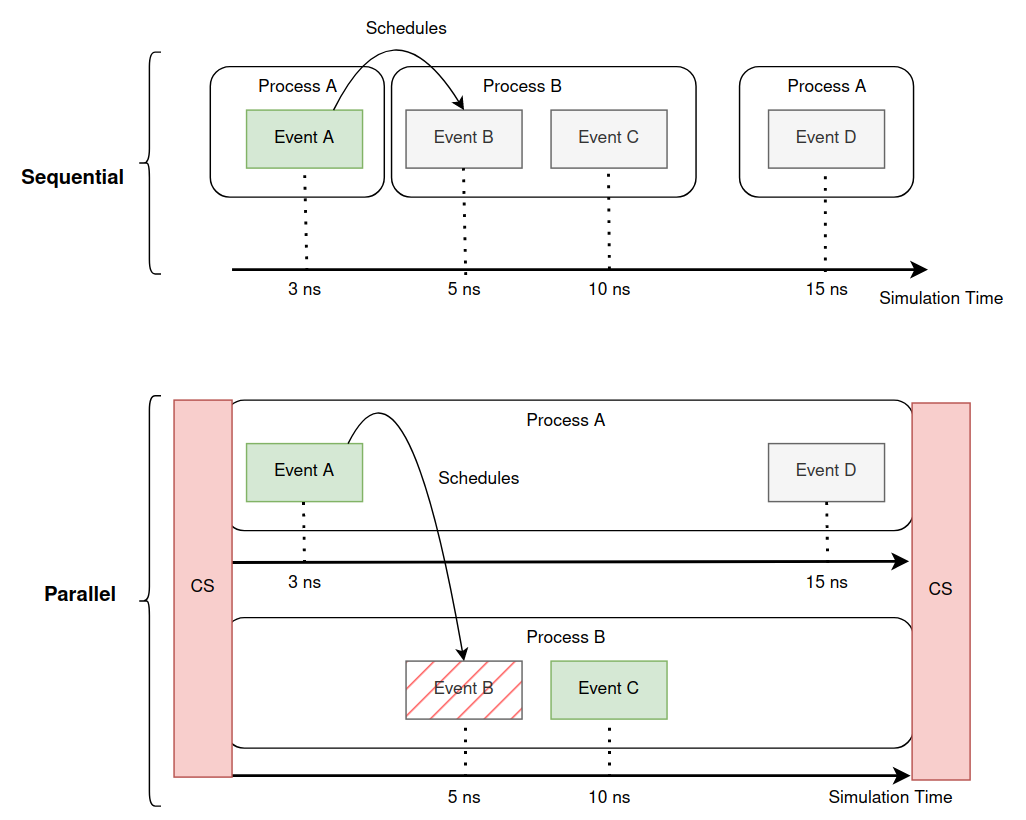
\includegraphics[width=0.85\linewidth]{Images/CausalityError.png}
 	\caption{The causality problem}
	 \label{fig_causalityError}
\end{figure}

When the simulation starts, event A is executed. Meanwhile, it triggers event B, which has an event timestamp of five nanoseconds. In the 
sequential mode, since it executes one event at a time, this is not a problem. In the parallel version, it can be, because each execution 
thread has its own time. Can happen that one thread is ahead of another, e.g. thread 1, which is executing process A, is at three nanoseconds, 
and thread 2, which is executing process B, is at ten nanoseconds, and when event A schedules event B to five nanoseconds, this event will 
not be executed for the reason that a \gls{des} cannot execute events in the past. On top of that, as mentioned before, if event B modifies 
the state variables of event C, the problem arises. 

The usage of \gls{td} in both modes, may increase the occurrence of causality errors. Not only that, it can create this type of error in 
another way. Take the coming scenario as an example. A simulator uses the parallel mode to test a system that is writing values into a 
\gls{dac} to play a song in an analog speaker, and, at the same time, solve complex mathematical equations to perform that audio. Supposing 
the wanted output frequency was the gold standard audio (44.1 kHz) \cite{audio}, the associated event needed to update the \gls{gpio} port 
every 2.27 microseconds. If the defined quantum is higher than that value, the event will not be executed at this event timestamp. Hence, 
the causality error was caused by the chosen quantum time. In this particular example, the consequence would be the production of audio 
that differs from the expected output. Although, in other cases, these errors can break the system functionality and crash the simulator. 

As peer with Fujimoto in \cite{PDESfujimoto}, there are two mechanisms to solve the problem: optimistic and conservative methods. In the 
first one, causality errors are not prevented at all, although they use detection and recovery strategies to correct that. The correction can 
be done with a rolling back method, which returns the simulation to a point before the causality error and sets the tighter synchronization. 
A problem with this method is the performance cost, because of this rewind in the simulation. The second option, on the other hand, avoids the 
possibility of any occurrence of these errors. An evaluation is done on the event, thus can be identified if the event is safe to process, that 
is, it is ensured that all events that should influence the given event have been processed before its execution. Some works with optimist 
approaches are \cite{busnot2020standard} and \cite{optimist2}. For \cite{dist-gem5} and \cite{asynchronousSimulator} are used conservative methods.

\section{Gem5}

One available \gls{fss} used in academia and industry is the Gem5 simulator \cite{TheGem5Simulator}\cite{Thegem5simulatorV2}. It had its roots 
in 2011, from the merge between M5 \cite{TheM5Simulator}, a \gls{cpu} simulation framework, and the multifacet \gls{gems} toolset \cite{TheGEMS}. 
With this combination, it is possible to use the best of both frameworks, the effective support of multiple \glspl{isa} and the cache memory 
and cache coherence models. It is also the result of the work between AMD, ARM, HP, MIPS, Princeton, MIT, the Universities of Michigan, Texas, 
Wisconsin, and many other institutions.

In addition, Gem5 came to overcome a demand in the market at the time. The main highlights are the flexible framework for researchers to 
evaluate their design in several different ways; Licensing terms that allow researchers and academia to work together without the pressure 
of revealing the proprietary information, in the industry case, or not getting credits for their contributions; Defined code style that ensures 
the code quality remains good so new collaborators understand faster and better the code \cite{TheGem5Simulator}. 

This section will explain in detail what are its capabilities and how can it be used. Then will be presented a work done by the \gls{ice} team 
of the \gls{rwth} Aachen University, which will be the reference work for this dissertation. To conclude, other simulators will be given to 
have a wide perspective of what exists in the market and when and where one can be better than another. 

\subsection{Overview}

Gem5 is a \gls{des} platform that has as its main goal to be a community tool focused on architectural modeling. It has a set of \gls{cpu} 
models and memory systems, and two different system modes, the \gls{se} and \gls{fs}. \autoref{fig_tradeoffTable} represents the different 
simulation configurations regarding the trade-off between speed and accuracy. 

\begin{figure}[H]
	\centering
 	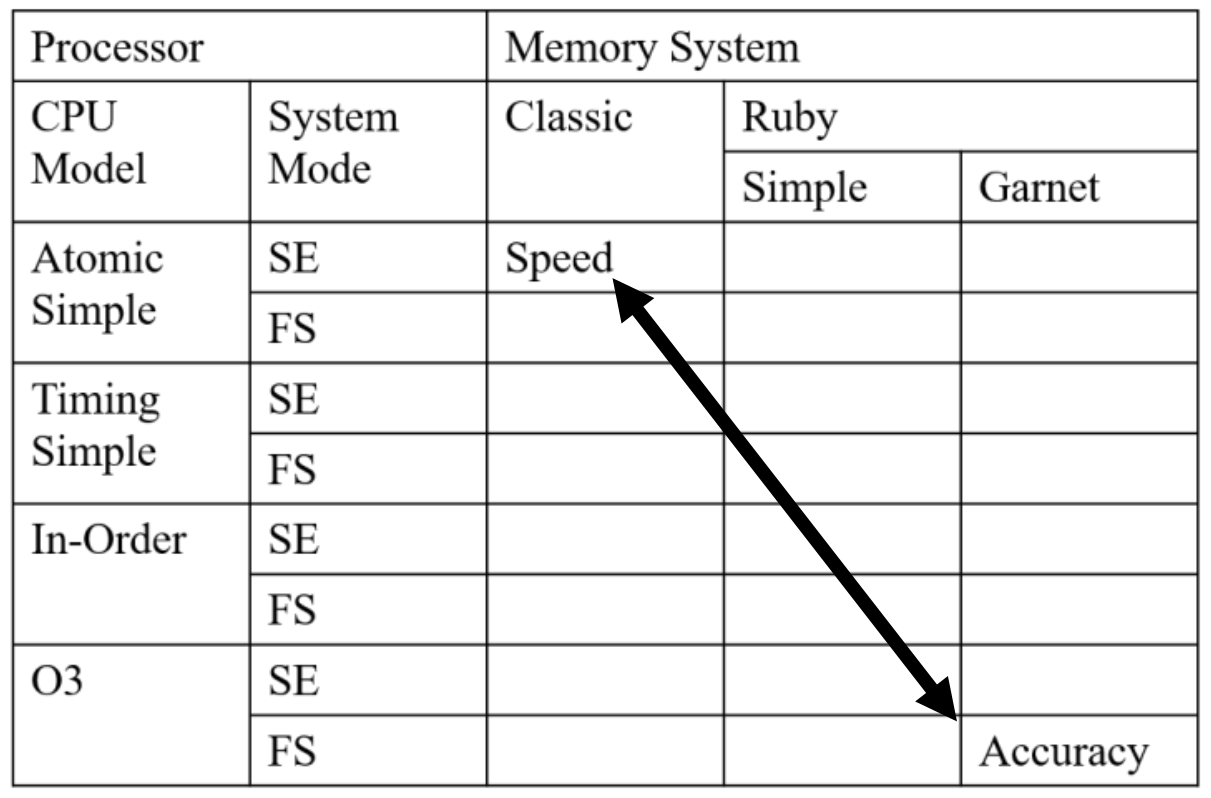
\includegraphics[width=0.6\linewidth]{Images/tradeoffTable.png}
 	\caption{Speed vs. accuracy spectrum \cite{TheGem5Simulator}}
	 \label{fig_tradeoffTable}
\end{figure}

As mentioned in the introduction of this section, one characteristic of Gem5 is flexibility. Several simulation configurations allow an 
adaptation to fit the requirements of the project or the level of wanted detail. A project where scalability is a must-have feature, for 
example, will not require a detailed \gls{cpu} model. The \gls{cpu} models will be explained with more detail in \autoref{subsec::SimCap}. 

In this simulator, components can be rearranged, parameterized, extended, or replaced easily to suit the project's needs. This is possible 
thanks to its pervasive object-oriented design, with the mix of Python and C++. All major components, like the memory, are SimObjects and 
share common behaviors for configuration, initialization, statistics, and serialization. Moreover, a user can create a customized SimObject, 
increasing even more the flexibility. To do that, it is required to define in a Python file the SimObject’s parameters, such as instantiation, 
naming, etc., and in the C++ files define its behavior.

Another remarkable characteristic is the support of different \glspl{isa}, counting with Alpha, ARM, SPARC, MIPS, POWER, x86, and recently 
RISC-V. Currently, not all possible combinations of ISAs and other components are known to be functional, as demonstrated in the 
\autoref{tab_ISAsupport}

\begin{table}[H]
\centering
\begin{tabular}{llll}
\cline{1-3}
\multicolumn{1}{|l|}{\cellcolor[HTML]{9B9B9B}\textbf{ISA}} & \multicolumn{1}{l|}{\cellcolor[HTML]{9B9B9B}\textbf{Level of ISA support}} & \multicolumn{1}{l|}{\cellcolor[HTML]{9B9B9B}\textbf{Full-system OS support}} &  \\ \cline{1-3}
\multicolumn{1}{|l|}{Alpha} & \multicolumn{1}{l|}{High} & \multicolumn{1}{l|}{Linux} &  \\ \cline{1-3}
\multicolumn{1}{|l|}{ARM} & \multicolumn{1}{l|}{High} & \multicolumn{1}{l|}{Linux, BSD, Android} &  \\ \cline{1-3}
\multicolumn{1}{|l|}{MIPS} & \multicolumn{1}{l|}{Low} & \multicolumn{1}{l|}{None} &  \\ \cline{1-3}
\multicolumn{1}{|l|}{Power} & \multicolumn{1}{l|}{Low} & \multicolumn{1}{l|}{None} &  \\ \cline{1-3}
\multicolumn{1}{|l|}{RISC-V} & \multicolumn{1}{l|}{Medium} & \multicolumn{1}{l|}{None} &  \\ \cline{1-3}
\multicolumn{1}{|l|}{SPARC} & \multicolumn{1}{l|}{Low} & \multicolumn{1}{l|}{None} &  \\ \cline{1-3}
\multicolumn{1}{|l|}{x86} & \multicolumn{1}{l|}{Medium} & \multicolumn{1}{l|}{Linux, BSD} &  \\ \cline{1-3}
 &  &  & 
\end{tabular}
\caption{Overview of the supported architectures in Gem5 \cite{hempelsimulation}}
\label{tab_ISAsupport}
\end{table}

Furthermore, it is also possible to simulate more than one computer system in various ways. It is done by instantiating another system and 
connecting it via a network interface, creating a client/server pair that communicates with the TPC/IP protocol. The results of the simulation 
remain deterministic, in other words, a particular input will produce always the same output. 

Gem5 uses other tools to perform specific jobs. The most important ones are the pybind11 \cite{jakob2019pybind11}, a lightweight header-only 
library that exposes C++ types in Python and vice versa, and SCons \cite{knight2002scons}, an open-source software construction tool that 
orchestrates the construction of software in a way that solves several problems compared to the other build tools. With the SCons scripts 
present in Gem5 is possible to build different binaries for different purposes. 

\begin{itemize}
    \item \textbf{Debug:} This mode has no optimizations, and thus it is the slowest one. It is mostly used when the opt version does not 
	provide enough detail in the debug session. 

    \item \textbf{Opt:} It has most of the available optimizations but still with same debug information. Compared to the debug version, it 
	is much faster.

    \item \textbf{Fast:} The fastest binary available. All optimizations are on, and there are no debug symbols. In addition, asserts are 
	removed, although panics and fatals are still included. This binary should only be used when it is desirable for maximum performance, and 
	the code is very unlikely to have bugs.
\end{itemize}

\subsection{Simulation Capabilities}
\label{subsec::SimCap}

As shown in the \autoref{fig_tradeoffTable}, this simulator provides different features that should be used regarding the project requirements. 
Those are the support for different \glspl{isa}, \gls{cpu} models, and execution modes. Also, it has the capability of modeling multiple systems 
at the same time, supports multiple devices, two different network models, and different cache coherence protocols \cite{TheGem5Simulator}.

While the event queue is responsible for executing its associated events, the \gls{cpu} is answerable to schedule the events thereby, it is 
possible to keep running the simulation even if no \glspl{cpu} are working. There are four types of \gls{cpu} models. Atomic simple, timing 
simple, in-order, and \gls{o3}. The atomic and timing models are the simplest ones. The main difference between them can be seen in 
the figures below. Meanwhile the first completes all memory accesses immediately, which makes it a proper option for tasks like 
fast-forwarding (a technique used to warm up micro-architectural state), the timing mode models the timing of memory accesses, providing a more 
accurate simulation.

\begin{figure}[H]
	\centering
 	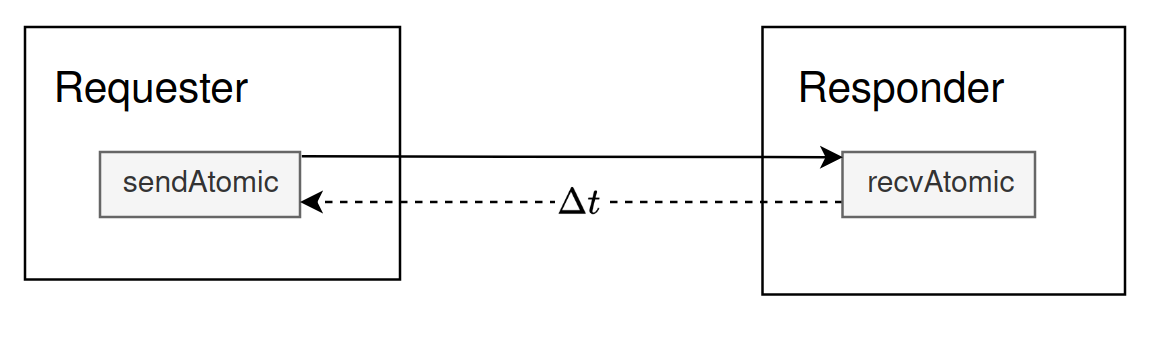
\includegraphics[width=0.7\linewidth]{Images/AtomicMode.png}
 	\caption{Atomic mode}
	 \label{fig_AtomicMode}
\end{figure}

\begin{figure}[H]
	\centering
 	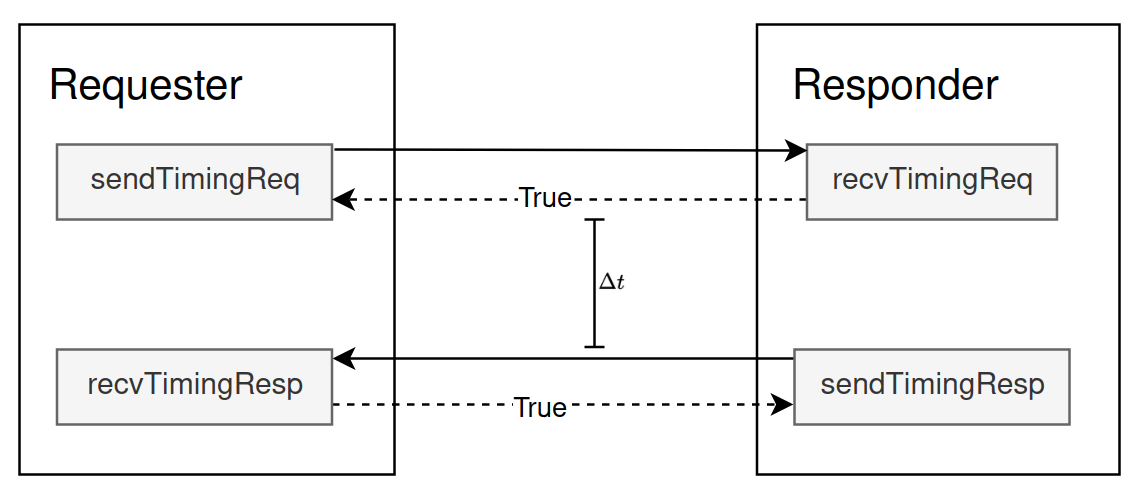
\includegraphics[width=0.7\linewidth]{Images/TimingMode.png}
 	\caption{Timing mode}
	 \label{fig_TimingMode}
\end{figure}

The in-order and O3 models are "execute-in-execute" models, which means that instructions are executed only in the execute stage once all 
dependencies have been resolved. For this reason, those are highly accurate.

Gem5 can operate either in \gls{fs} and \gls{se} mode. The \gls{fs} is more complex and complete, in a way that it supports interrupts, 
exceptions, \gls{io} devices, and so on. As the name suggests, the \gls{se} simulates system calls, like write(). This characteristic can 
be a bottleneck to multi-thread applications nevertheless, results in a faster simulation. If the workload has lots of \gls{io} iterations or 
\gls{os} services, the \gls{fs} is the proper choice, otherwise the \gls{se} may be considered, even because some \glspl{isa} do not support 
the \gls{fs} mode yet. 

Another important capability is the support to the classic and ruby memory system, due to the integration of both works (M5 and GEMS). On one 
hand, the classic system is fast and easy to configure. On the other hand, the ruby system is more flexible and accurate. Gem5 also offers an 
extension for the simple version named Garnet. At the time, Gem5 supports HeteroGarnet or Garnet 3.0 which brings improvements compared to the 
previous version, for example, it can enable accurate simulation of emerging interconnect systems. 

%Ver o paper das cache

Even though Gem5 is a very flexible simulator, according to \cite{TheGem5Simulator}, there are other capabilities the developers want to 
include. A first-class power model, full cross-product \gls{isa}/\gls{cpu}/memory system support, and parallelization are some examples. 
It is evident that there is still much work to be done, but compared to the first review, there are lots of advances and improvements, like 
the support for the RISC-V architecture and the \gls{kvm} \cite{Thegem5simulatorV2}. 


%CPU, memory, cache, ISAs, Execution modes, Devices
%Diferentes modes para diferentes propositos
% Falar sobre caches - para o problema dos simulações xD

\subsection{Usage}

To start using Gem5 it is necessary two things. First of all, the simulator's binary for the wanted \gls{isa} is necessary. As mentioned before, 
there are three different types of binaries, therefore it should be chosen mindfully. Then, it is mandatory the definition of the system. 
It describes the components comprising the \gls{soc} and details their interconnections. 
Gem5 provides in its tutorials the simplest system a developer can use, and it is presented in the following picture.

\begin{figure}[H]
	\centering
 	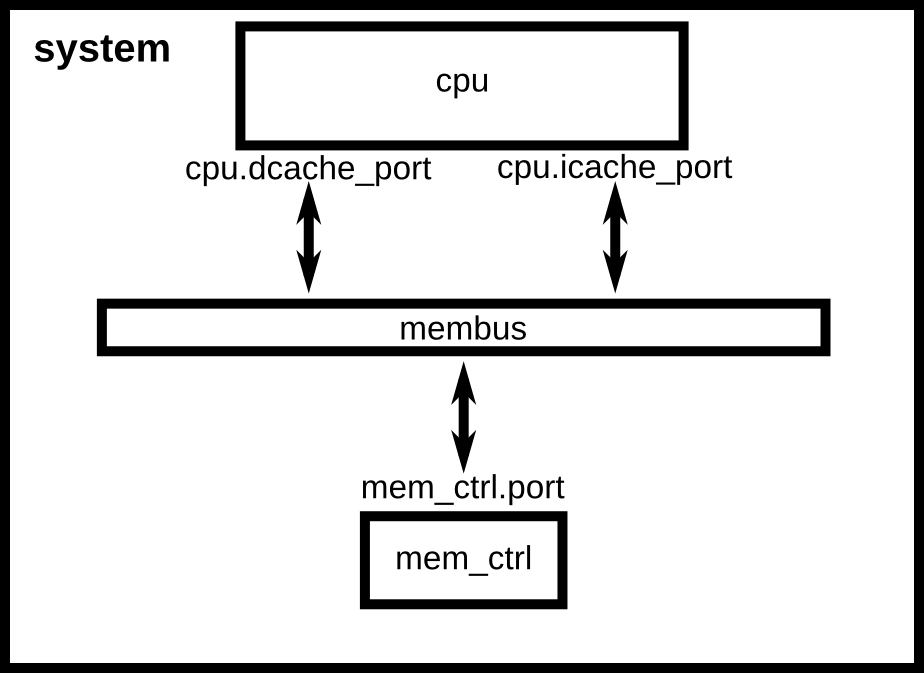
\includegraphics[width=0.5\linewidth]{Images/simple_config.png}
 	\caption{Simple system configuration diagram}
	 \label{fig_simple_config}
\end{figure}

All the configuration is performed in a Python script, while the functionality of the simulator is implemented in C++. Making changes to the 
latter requires creating a new binary, whereas in the former case, it does not. The next code demonstrates the instantiation 
required in the Python script to execute the simulation

\pagebreak

\begin{lstlisting}[language=Python, caption=Script to instantiate and execute the simulation]
    #create the system to simulate
    system = MySystem ( opts )

    #set up the root SimObject and start the simulation
    root = Root(full_system = False, system = system)
    m5.instantiate()

    #instantiate all objects above
    print("Beginning simulation!")
    exit_event = m5.simulate()

    #After execution
    print('Exiting @ tick {} because {}'
      .format(m5.curTick(), exit_event.getCause()))

\end{lstlisting}

Finally, to run Gem5, the command should first have the directory of the binary, and then the directory of the script. Furthermore, it can 
have more arguments to specify the system or the simulation modes, e.g. the \gls{cpu} model.

\subsection{Par-gem5}
\label{subsec:pargem5}

A huge problem of Gem5 is its speed. At the moment, its official version only offers a single-threaded simulation. Even with the best 
\gls{cpu} or the fastest memory on the host machine, the simulation can not get close to one \gls{mips}, which results in long execution 
times. For instance, while the SPEC2017 integer benchmark can take ten minutes in a host computer, with Gem5 the same workload can take more 
than two years \cite{pargem5}. As referred in the \autoref{subsec::SimCap}, parallelize Gem5 is one desired feature to have however, more than 
ten years passed and there are no developments on this topic, only the support for \gls{kvm}. 

Par-gem5 \cite{pargem5} arises to solve this problem. It was developed by the \gls{ice} team of the \gls{rwth} Aachen University, with the 
collaboration of Huawei. It utilizes the multi-threading capabilities of the host system through a modified conservative, synchronous 
\gls{pdes} approach, which allows the execution to be dispatched to multiple simulation threads that run independently from the rest of 
the system for a time $t_{\Delta q}$ - the so-called quantum or quanta. At the time, only dist-gem5 \cite{dist-gem5}, a work that focuses 
on simulating distributed systems connected via a \gls{nic}, has implemented a parallel extension. Nonetheless, its application is very strict, 
since can only be used in this type of system thus, par-gem5 comes to overlap this problem and be a generalized parallel version.

In the initialization phase, each \gls{cpu} is assigned to a dedicated event queue, and all other objects are assigned to the default event 
queue (q0). Thereby, the total number of threads will be the number of cores plus one. This version cannot be classified either as conservative 
or optimistic for the reason that it allows causality errors to occur.

\begin{figure}[H]
	\centering
 	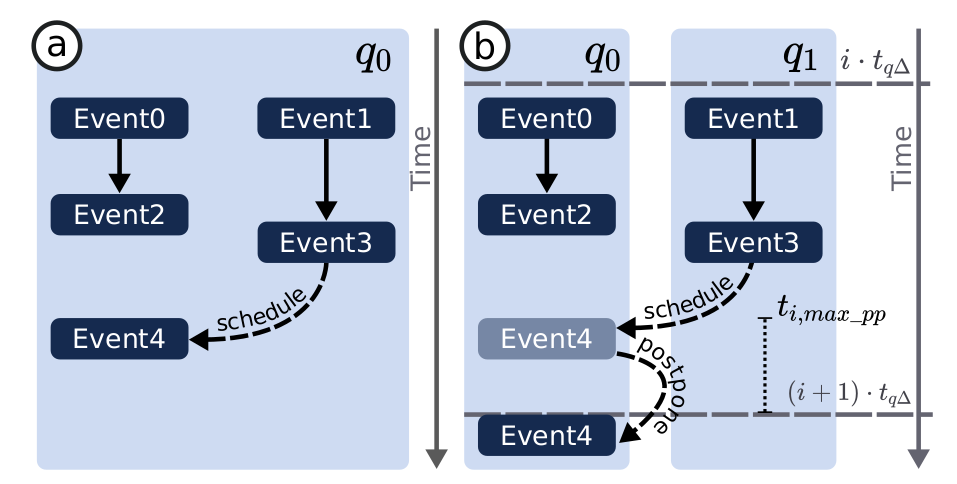
\includegraphics[width=0.7\linewidth]{Images/SchedulingEventGem5.png}
 	\caption{Example of scheduling events in Gem5 \cite{pargem5}}
	 \label{fig_SchedulingEventGem5}
\end{figure}

Scenario A represents the typical sequential simulation, and scenario B the par-gem5 scheduling method. When an event is scheduled to another 
\gls{cpu}, it can either be executed or postponed to the following synchronization. The event is postponed when its timestamp has passed. 
Consequently, it can lead to a chronologically incorrect execution order of events, affecting the simulation's accuracy, or in the worst case, 
flaws in the functionality of the simulated system. Nevertheless, in \cite{pargem5} is proven that the inaccuracy can be kept within a single-digit 
percentage.

The results of this work were very positive. For example, a speedup of 24.7x was achievable without losing accuracy significantly. Moreover, 
it has been demonstrated that there exists a saturation point in the definition of the quantum. Based on their tests, this point falls between 
ten and a thousand microseconds, indicating that increasing the quantum beyond this range does not result in performance gains. Another 
important conclusion was the relationship between cores and inaccuracy. If the quantum does not change, when the number of cores increases, the 
inaccuracy also increases. 

One way to solve the problem is to set a smaller quantum, but getting the perfect quantum is hard. One can be perfect for one benchmark and 
bad for another simultaneously. Zurstraßen et al. \cite{BeyondQuantumTDSim} go further and perform a study where this trade-off is evaluated. 
In the end, it was concluded the speedup of the simulation as a function of the quantum behaves similarly to a sigmoidal or "S"-shaped curve, while 
the simulation inaccuracy, on the other hand, grows linearly. Moreover, for the cases studied, 95\% of the maximum attainable speedup was 
obtained at a quantum between 1000 and 10000 instructions, as different quantums suit better for different workloads.

Finding a quantum that allows high accuracy with high speedup is one of the main challenges when running a \gls{pdes}. There are some works 
that try to explore this problem and come up with solutions, but none of them at the moment, as shown in the table below, is generalized, 
real-time, and for \gls{pdes} simultaneously. 

\begin{table}[H]
\centering
\begin{tabular}{ccccl}
\cline{1-4}
\multicolumn{1}{|c|}{\cellcolor[HTML]{9B9B9B}\textbf{Work}} & \multicolumn{1}{c|}{\cellcolor[HTML]{9B9B9B}\textbf{Real-Time}} & \multicolumn{1}{c|}{\cellcolor[HTML]{9B9B9B}\textbf{Supports PDES}} & \multicolumn{1}{c|}{\cellcolor[HTML]{9B9B9B}\textbf{Generallized}} &  \\ \cline{1-4}
\multicolumn{1}{|c|}{Jung et al. \cite{optimist2} (2019)} & \multicolumn{1}{c|}{X} & \multicolumn{1}{c|}{} & \multicolumn{1}{c|}{X} &  \\ \cline{1-4}
\multicolumn{1}{|c|}{Glaser et al. \cite{GlaserTD} (2015)} & \multicolumn{1}{c|}{X} & \multicolumn{1}{c|}{} & \multicolumn{1}{c|}{X} &  \\ \cline{1-4}
\multicolumn{1}{|c|}{Jünger et al. \cite{optimizingTD} (2021)} & \multicolumn{1}{c|}{} & \multicolumn{1}{c|}{X} & \multicolumn{1}{c|}{X} &  \\ \cline{1-4}
\multicolumn{1}{|c|}{dist-gem5 \cite{dist-gem5}} & \multicolumn{1}{c|}{X} & \multicolumn{1}{c|}{X} & \multicolumn{1}{c|}{} &  \\ \cline{1-4}
\multicolumn{1}{l}{} & \multicolumn{1}{l}{} & \multicolumn{1}{l}{} & \multicolumn{1}{l}{} & 
\end{tabular}
\caption{Overview of the different works regarding the quantum definition}
\label{tab_OverviewDynamicQuantum}
\end{table}

The first work uses a technique that tries to achieve 100\% accuracy by rectifying causal errors when they happen, forcing the system to 
simulate again the faulty part with a smaller quantum. This approach is called a rollback mechanism. One of the best-known methods of this 
type is the “Time
Warp algorithm” \cite{jefferson1985virtual}. Despite this concept is not new, it is still very present nowadays \cite{busnot2020standard}. 
Beyond the non-\gls{pdes} support, a criticism of this method is the performance cost. Because it "rolls back" the simulation every time a 
causality error happens, the execution time will be much higher.

The second work uses a wiener filter to update the quantum within the simulation. This work was able to obtain great performance since it 
does not require lots of computational resources. Here, there are two simulators, SystemC, and Verilog, that communicate between them by 
a \gls{adc}. Hence, the quantum that leads to high accuracy should be equal to the smaller latency. To get that, it assumes a stationary 
process and model order is known, which sometimes is not possible. Moreover, this work is done in the context of a single-threaded simulation, 
so there is no \glspl{ipc} being evaluated.

In the context of \gls{pdes}, Jünger developed a method whose principle is to classify events as relevant or irrelevant. An event is considered 
irrelevant to others if its synchronization is not related to them, for example, a timer interrupt. With this information, each local quantum is 
adapted accordingly to the following event. In consequence of that, it is possible to obtain perfect accuracy, without performance costs. To do 
this classification, firstly the simulation must be run, and then with the results, the events can be classified. This makes the technique not so 
desirable since the user needs to execute twice the same workload. 


\subsection{Other Simulators}

%Integrar isto
%https://community.arm.com/arm-research/b/articles/posts/running-trusted-firmware-a-on-gem5

Like Gem5 other simulators are used for the same purpose. This subsection will discuss some of them, their advantages and disadvantages 
compared to the simulator under study, to have a better perspective of what is offered about this subject at the moment. 

Starting with QEMU (Quick EMUlator) \cite{theQEMUsimulator}, as the name suggests, it is a versatile full-system emulator that can emulate 
various architectures, including x86, ARM, PowerPC, and more. As explained earlier in the \autoref{subSec::EmbeddedSim}, there is a difference 
between an emulator and a simulator, yet QEMU was considered due to other similarities, like the open source availability, the support to 
different architectures, and the active development community. José Morales in \cite{morales2016evaluating} compared these two simulators in 
detail and, in the end, the conclusion of his study com be summed up in the next figure.

\begin{figure}[H]
	\centering
 	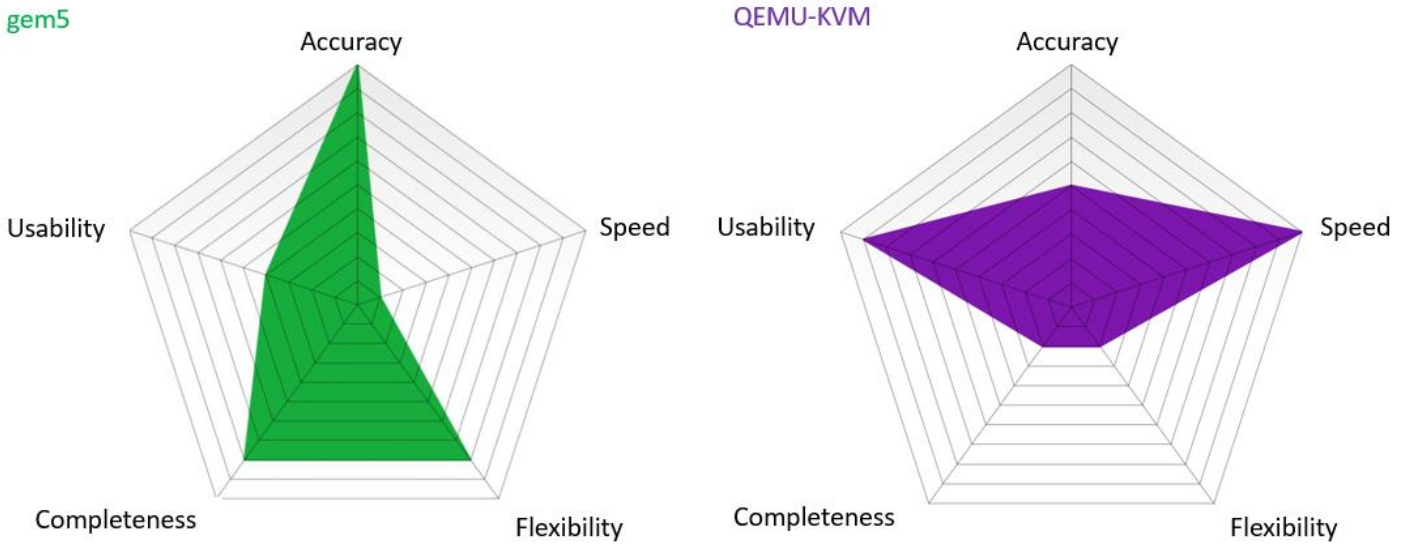
\includegraphics[width=0.8\linewidth]{Images/gem5VSQEMU.png}
 	\caption{Final assessment charts \cite{morales2016evaluating}}
	%\label{fig_gem5VSQEMU}
\end{figure}

One characteristic of QEMU is its loosely timed coding style, which provides high simulation speed environments. Cycle-accurate coding style, 
as \gls{rtl} simulators, on the other hand, cover fine-level \gls{ip} tuning. This is useful to validate hardware design. Gem5 can be positioned 
within the spectrum as an intermediate solution, offering a balance between performance and power exploration for early system-level solutions.

\begin{figure}[H]
	\centering
 	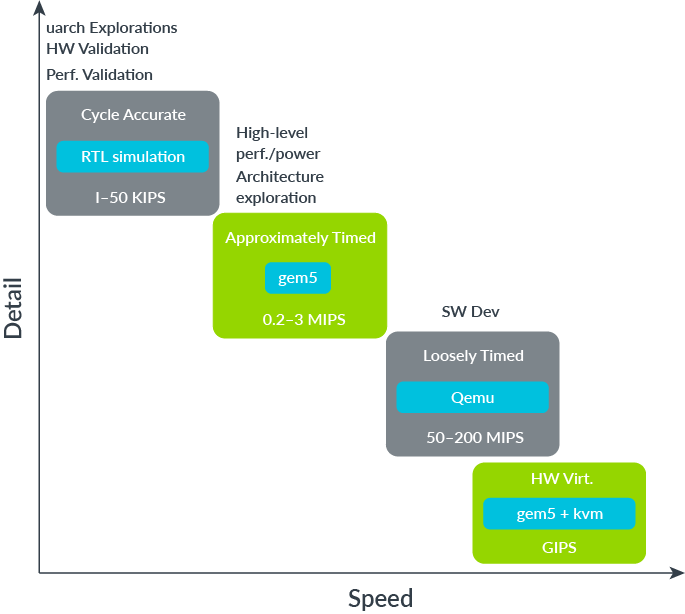
\includegraphics[width=0.6\linewidth]{Images/SimulationComparation.png}
 	\caption{ Modelling solutions spectrum \cite{herrera2020running}}
	%\label{fig_gem5VSQEMU}
\end{figure}

Another platform already mentioned is SystemC \cite{systemC}. It is a set of C++ classes and macros which provide an event-driven simulation 
interface for system and hardware design. Its main purpose is to provide a C++-based standard for designers and architects who need to address 
complex systems that are a hybrid between hardware and software. Furthermore, it can be used also as an \gls{hdl}, still, it may require an 
evaluation due to its syntactical overhead compared to other options like Verilog or VHDL. It also supports \gls{tlm}-2.0, which allows us to 
model the communication as function calls. Events are applied to an entire transaction payload, rather than to individual bus signals, and at 
the protocol phase
boundaries, rather than at clock edges \cite{wieman2012overview}. Thus, the simulations have much better performance, 100-10000 times faster, 
when compared to the cycle-accurate version. The main advantages are its standardization in the industry, lots of documentation and work, and 
the capability to quickly simulate hardware and software systems on different levels of abstraction. Contrarily, it is not so flexible hence, 
it requires external modules to complement itself, e.g., it can not perform cycle-accurate simulations, and most of the modules/\glspl{ip} are 
not free of charge, meaning extra costs. 


Ayaz Akram and Lina Sawalha developed a work where a comparison of x86 computer architecture simulators is done \cite{akram2016comparison}. In 
this study are evaluated four simulators: Gem5 \cite{TheGem5Simulator}, Multi2Sim \cite{ubal2012multi2sim}, Sniper \cite{carlson2011sniper}, 
and PTLsim \cite{yourst2007ptlsim}. The authors selected these simulators based on their diverse design approaches regarding the level of 
detail and abstraction. All of them are modern simulators that are actively being developed, except for PTLsim, which is currently not 
undergoing active development but is still widely utilized. The following image presents a features comparison between the previous simulators 
and ZSim \cite{sanchez2013zsim}. 

\begin{figure}[H]
	\centering
 	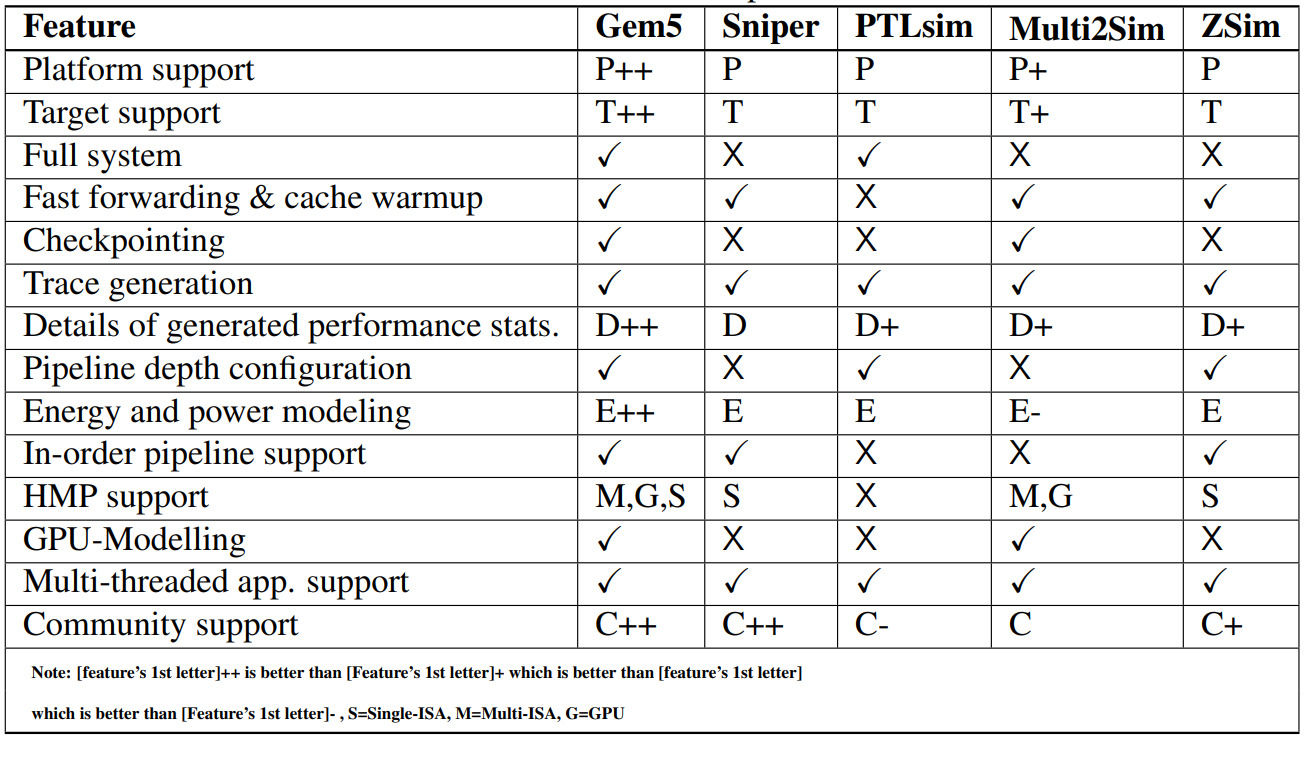
\includegraphics[width=0.7\linewidth]{Images/ComparationTableSimulators.png}
 	\caption{Feature comparison between simulators \cite{akram2016comparison}}
	 \label{fig_ComparationTableSimulators}
\end{figure}

In their work, these platforms were tested with three different benchmarks. In the end, was possible to conclude that Gem5 is a good option 
when very detailed results and multiple \glspl{isa} support are wanted. Sniper is specifically designed for multi-core simulations and is 
considered the most accurate among the simulators examined. However, it lacks the capability to generate detailed performance statistics for 
the simulated system and is comparatively less flexible than the other simulators. Then, if the focus is a CPU-GPU architecture simulation, 
Multi2Sim proves to be a great preference. Finally, PTLsim did not get a best-case scenario to be used nevertheless, it is the base of other 
x86 diverse simulators, such as the MARSSx86 simulator \cite{patel2011marss}.

\section{Machine Learning}

\glsxtrfull{ml} is at present-day an extremely important subject, encompassing applications in both smaller devices like watches and larger 
ones such as cars.  Autonomous driving is one example of what can be done with machine learning \cite{bachute2021autonomous}. Although this 
theme emerged recently, with the evolution of computers, it was first defined by Arthur Samuel in 1959, who states that 
\textit{ it is a field of computer science that gives computers the ability to learn without being explicitly programmed }\cite{samuel1959some}. 

There are various types of \gls{ml} algorithms, such as classification, error cancellation, and prediction. Depending on the project 
requirements, these algorithms can be utilized individually or combined in a manner that complements each other to address complex problems, 
like \cite{bachute2021autonomous}. The following picture shows some of the commonly used algorithms in \gls{ml}.

\begin{figure}[H]
	\centering
 	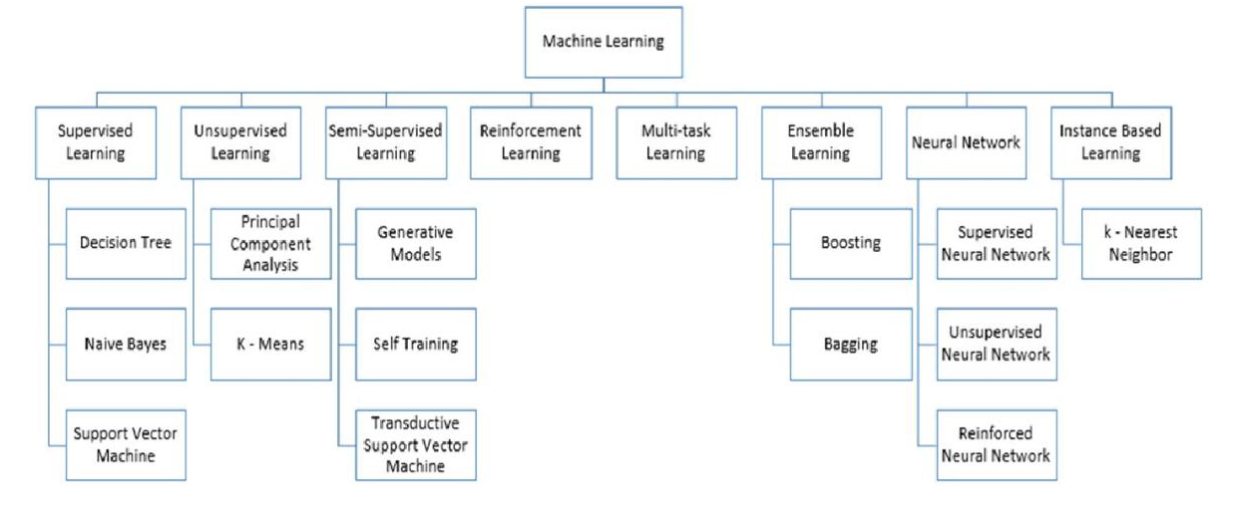
\includegraphics[width=0.9\linewidth]{Images/TypesOfML.png}
 	\caption{Examples of \gls{ml} algorithms \cite{mahesh2020machine}}
	 \label{fig_TypesOfML}
\end{figure}

Within this dissertation, only neural networks will be considered. They can be divided into \glsxtrfullpl{ann} and \glsxtrfullpl{bnn}. 
A \gls{bnn} is a network of neurons that are connected by axons and dendrites, and the connections between neurons are made by synapses. 
An \gls{ann} will be explained in detail in the next subsection. Also, it will be presented how \gls{ml} can be applied to simulation and the 
improvements it brought. 

\subsection{Artificial Neural Networks}

\glspl{ann} are types of \gls{ml} that are inspired by the operation of the human brain. They try to model it to implement a particular task or 
function of interest. To do that, the biological neuron was studied in detail to understand how it works. How the information flows from one 
to another, how it adjusts the importance of several inputs, and so on. \autoref{fig_ComparationBNN_ANN} and 
\autoref{tab_compararionBNN_ANN_table} represent how a biological neuron can be transformed into an artificial one.

\begin{figure}[H]
	\centering
 	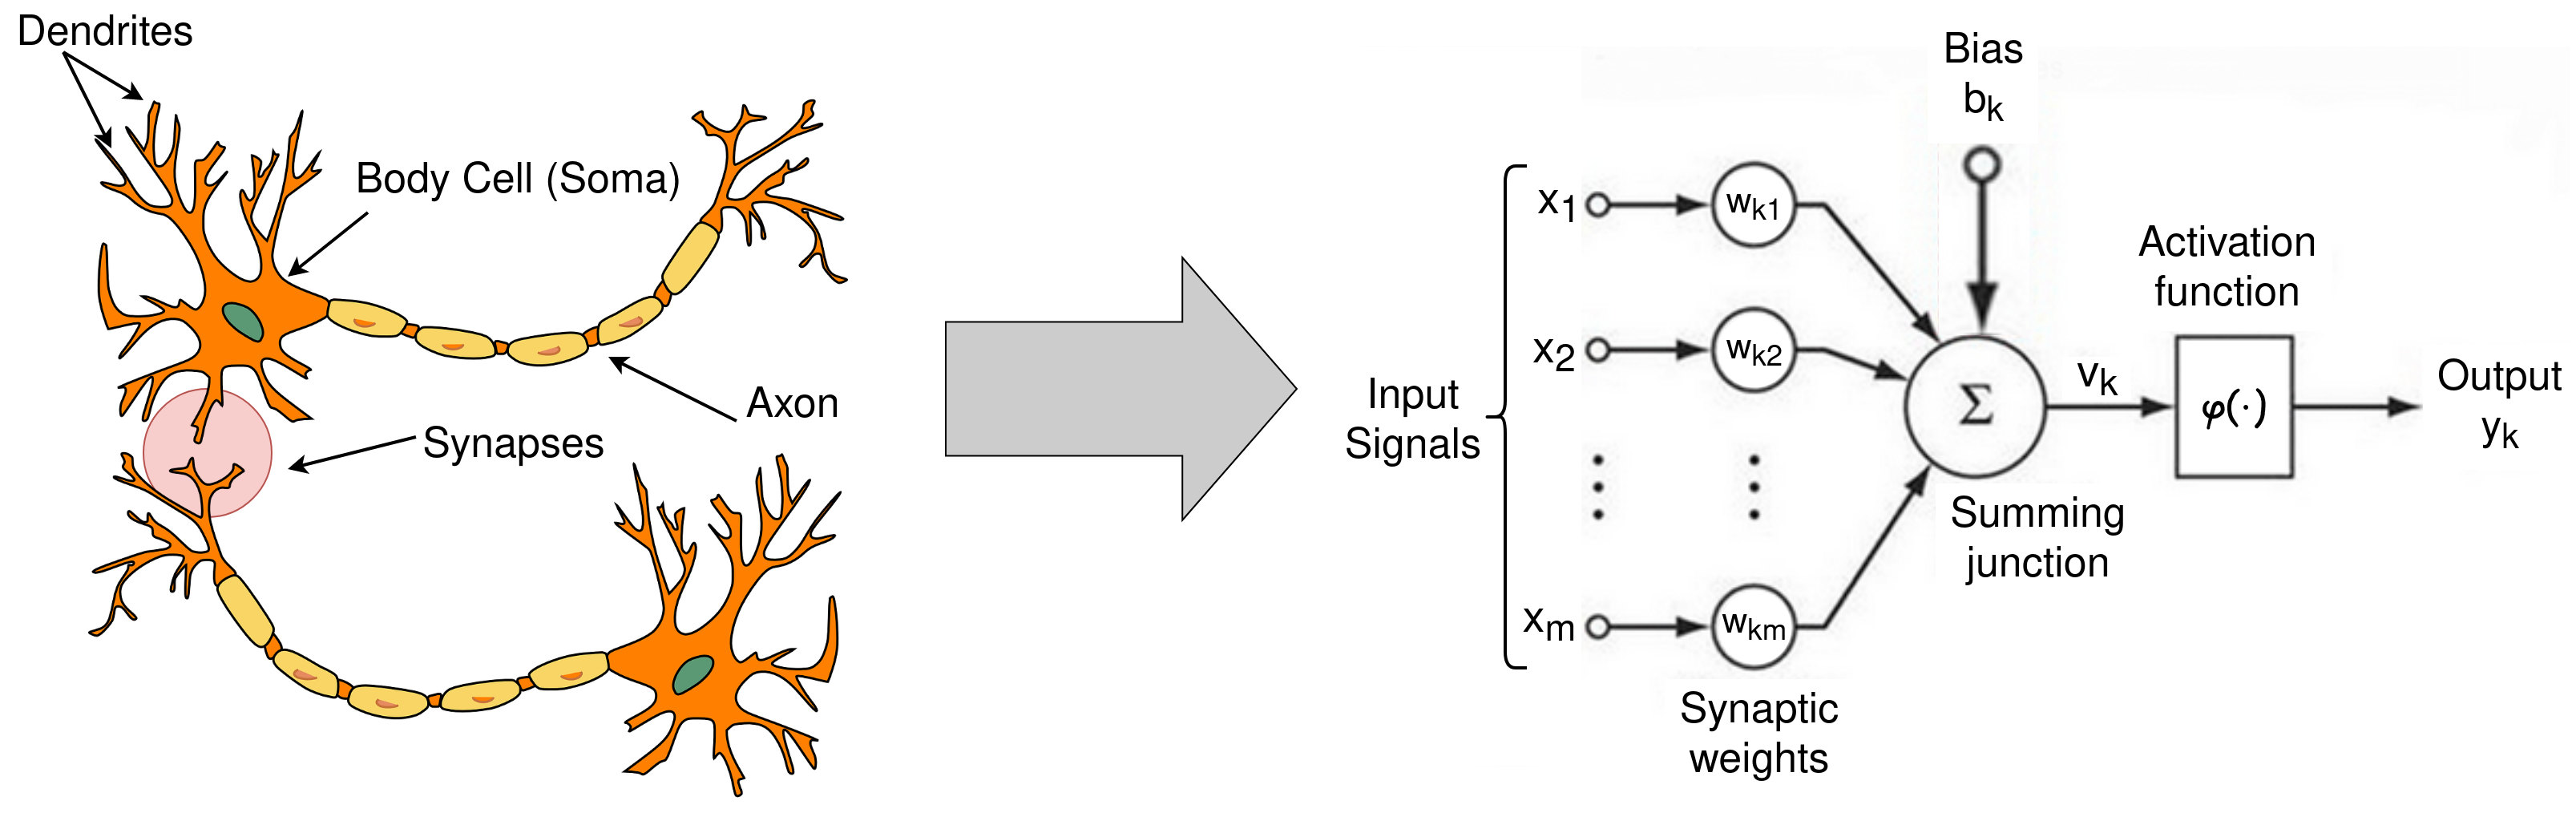
\includegraphics[width=0.9\linewidth]{Images/ComparationBNN_ANN.png}
 	\caption{Comparison diagram between a biological and an artificial neuron}
	 \label{fig_ComparationBNN_ANN}
\end{figure}

\begin{table}[]
\centering
\begin{tabular}{ccl}
\cline{1-2}
\multicolumn{1}{|c|}{\cellcolor[HTML]{9B9B9B}\textbf{BNN}} & \multicolumn{1}{c|}{\cellcolor[HTML]{9B9B9B}\textbf{ANN}} &  \\ \cline{1-2}
\multicolumn{1}{|c|}{Dendrites} & \multicolumn{1}{c|}{Inputs} &  \\ \cline{1-2}
\multicolumn{1}{|c|}{Soma / Body cell} & \multicolumn{1}{c|}{\begin{tabular}[c]{@{}c@{}}Summing and activation\\ junction\end{tabular}} &  \\ \cline{1-2}
\multicolumn{1}{|c|}{Synapses} & \multicolumn{1}{c|}{\begin{tabular}[c]{@{}c@{}}Weights or\\ interconnections\end{tabular}} &  \\ \cline{1-2}
\multicolumn{1}{|c|}{Axon} & \multicolumn{1}{c|}{Output} &  \\ \cline{1-2}
\multicolumn{1}{l}{} & \multicolumn{1}{l}{} & 
\end{tabular}
\caption{Comparison table between a biological and an artificial neuron}
\label{tab_compararionBNN_ANN_table}
\end{table}

Like the human brain, \glspl{ann} also needs to learn. There are three ways to train an \gls{ann}, which are also inspired by human actions. 
Supervised learning is a method that teaches the \gls{nn} by providing the outputs for certain inputs. The predicted outputs are compared to 
the real ones, and then weights are adjusted according to the error. In the real world, it can be compared to heating food. The human knows 
how warm wants his food, but he cannot calculate how much time should it be warming in the microwave. Thus, he makes a prediction, and based on 
what result, time may be redefined.

In the opposite way, unsupervised learning is a technique where the \gls{nn} only knows the inputs. The training is done only with the input 
information, which is a good solution for clustering or density problems, where the data is categorized based on similarities. A great example
is when it is required for a person to sort apples. Since there is no information, for instance, the person uses the color 
to distinguish them and perform the sort operation. 

The last method is the reinforced \gls{nn}. There is an agent that controls the outputs of the system. The \gls{nn} may receive a reward or a 
penalty for each action it performs. With this information, it adapts its behavior to receive the fewest penalties possible. A comparison can 
be made to a relationship between a mother and her son, where the mother supervises the actions of her son, and reward or alert him when he 
does something.

Also, \glspl{ann} can be classified into two different classes. The Feed-Forward \glspl{nn} and the Recurrent \glspl{nn}. In the first one, 
the information pursuers a linear path, where the output of one neuron will be the input of another. The other way around, the output of a 
neuron is used as input of the same neuron, which is appropriate for non-linear applications. 

\subsection{Learning Rules}

As illustrated in the \autoref{fig_ComparationBNN_ANN}, in an \gls{ann} the inputs, before summing, suffer an adjustment by the synaptic weights. 
To define these weights, learning rules are used, that is, self-adaptive equations that update the weights and bias levels of neurons, enabling 
a neural network to learn from its input data and enhance its performance. There are diverse types of learning \cite{haykin2009neural}. Some 
examples are:

\begin{itemize}
    \item Hebbian learning rule
    \item Perceptron learning rule
    \item Delta learning rule (Widrow-Hoff rule)
    \item Competitive/correlation learning rule (Winner-takes-all)
    \item Outstar learning rule (Grossberg learning)
\end{itemize}

For this thesis, only the delta learning rule or \gls{lsm} algorithm will be considered. It was introduced by Widrow and Hoff in 1960 in 
\cite{widrow1960adaptive}, and its objective is to minimize the sum of squares of the linear errors over the training set. Additionally, 
a typical neuron used in \glspl{nn} is the "ADAptive LInear NEuron" or ADALINE. It consists of an adaptive linear combiner cascaded with a 
hard-limiting quantizer, which generates a binary output (-1 or 1) used, e.g., for classification problems. A schematic can be seen in the 
figure below. If it is removed, the output will be analog, which may be useful, for instance, to noise-canceling applications 
\cite{widrow1985adaptive}. Further, it is possible to have multiple layers of neurons to address more complex systems (Multiple ADAptive 
LInear NEuron, or MADALINE).

\begin{figure}[H]
	\centering
 	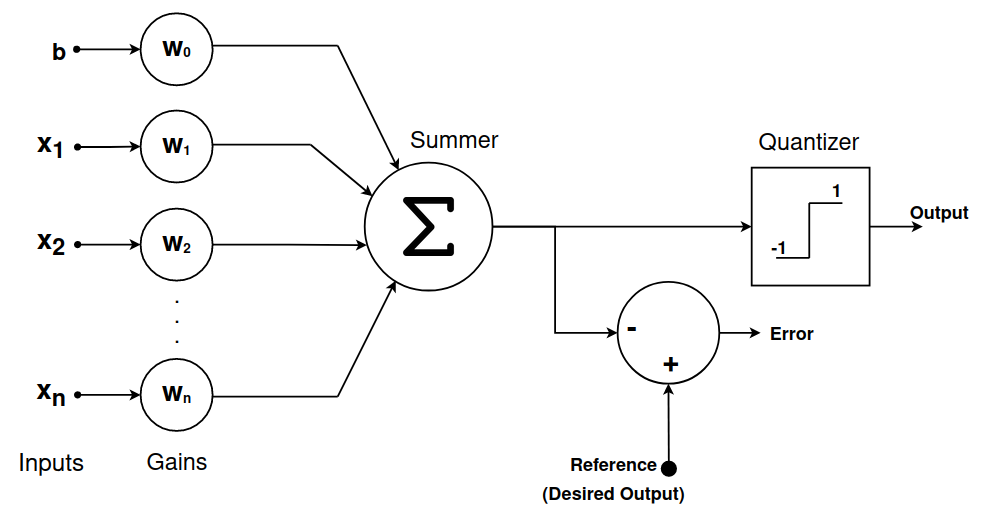
\includegraphics[width=0.8\linewidth]{Images/AdalineSquematic.png}
 	\caption{Schematic of ADALINE \cite{widrow1960adaptive}}
	 \label{fig_AdalineSquematic}
\end{figure}

The linear error is defined to be the difference between the desired response and the linear output. After that, this error signal is used 
to train the \gls{nn}, regarding the \autoref{eq_LSM} \cite{widrow1995perceptrons}.

\begin{equation}
    Wi_{k+1} = Wi_{k} + 2 \mu \varepsilon_{k}Xi_{k}
    \label{eq_LSM}
\end{equation}

Where $Wi$ is the weight associated with the input i, $k$ defines the time, $\mu$ is a parameter that controls stability, called learning 
rate, $\varepsilon_{k}$ is the linear error, and $Xi_{k}$ is the input i. 

\subsection{Machine Learning in Simulation}

\gls{ml} and simulation are two different topics that can complement each other. For example, when evaluating risk management, where the 
behavior of the system is based on causal relationships, hidden dependencies, etc. \cite{mitchell2017natural}, a combination of both worlds 
could be beneficial.  L. von Rueden in \cite{von2020combining} presents a work that defines three subfields when combining both, 
simulation-assisted \gls{ml}, machine-learning-assisted simulation, and hybrid.

\begin{figure}[H]
	\centering
 	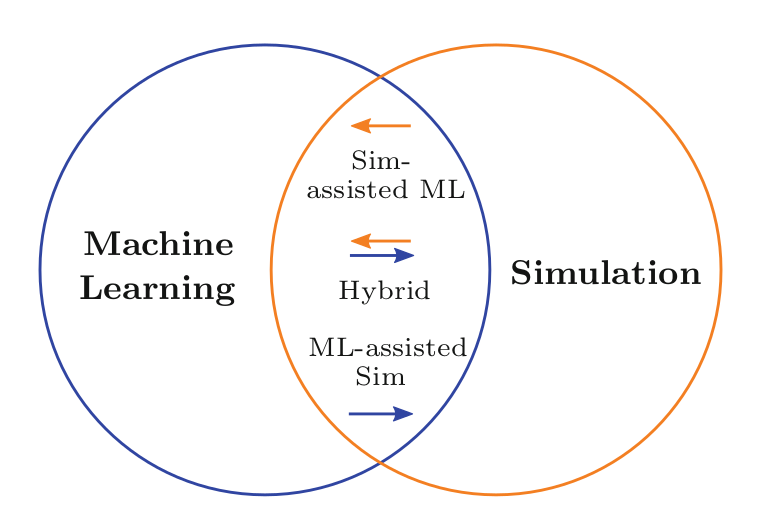
\includegraphics[width=0.5\linewidth]{Images/SimAndML.png}
 	\caption{Subfields of combining \gls{ml} and simulation \cite{von2020combining}}
	%\label{fig_AdalineSquematic}
\end{figure}

Machine learning in simulation is often used to detect patterns in data or support the solution process. It can integrate all four components 
of the simulation. These components are: model reduction \cite{benner2015survey}, input parameters \cite{tsymbalov2019deeper}, numerical 
method \cite{noe2020machine} and simulation results \cite{albertsson2018machine}. Because of this versatility, \gls{ml} is an important part 
of the simulation world and should be used to obtain better conclusions and performance. Yet, it is not being fully exploited, that is, 
simulations, especially in the industry, are run with very specific analysis goals, ignoring further analysis that could be interesting for 
other contexts \cite{von2020combining}.

\section{Co-Simulation}

The development of truly complex engineered systems that integrate physical, software and network aspects is on the rise \cite{gomes2017co}. 
The simulation of these all together is not reliable hence, the need to divide the system into different teams arises. Each one develops a 
part of the final solution, that, in the end, is integrated into the others. Different abstraction layers may demand distinct simulation tools, 
as some are finely tuned for specific domains, yielding results that closely mock real-world behavior. The \autoref{fig_DomainsComplexSystem} 
shows an example of different domains in a complex system. 

Normally, each part is tested and verified alone, that is, without iterations from other modules \cite{gomes2017co}. However, information on 
another part of the system may be needed, for example, a wave input to produce a sound. A possible solution can be the generation of local 
files containing the necessary information nevertheless, interactions are not thoroughly tested. This may create validation failures, which 
can result in delays in the development and extra costs in the development.

\begin{figure}[]
	\centering
 	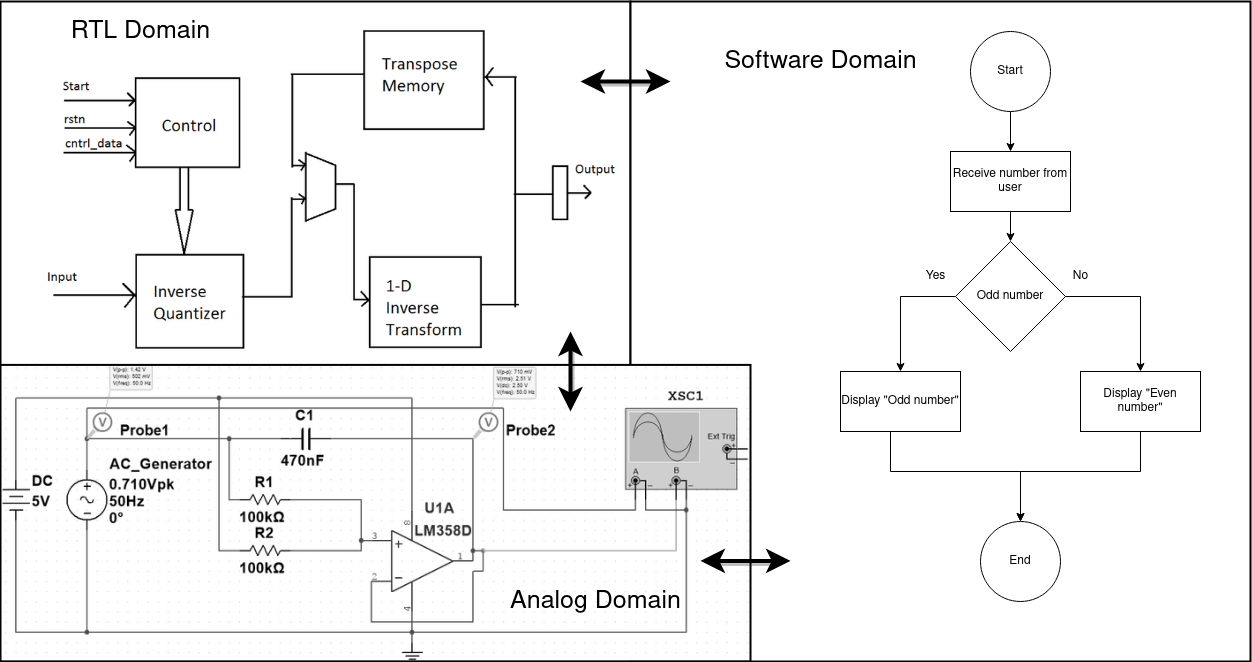
\includegraphics[width=0.9\linewidth]{Images/DomainsComplexSystem.png}
 	\caption{Different domains of a complex system}
	 \label{fig_DomainsComplexSystem}
\end{figure}

Co-simulation is proposed as a solution to overcome the latter issue \cite{gomes2017co}. It consists of a combination of simulators that 
execute concurrently, with one providing information to the others and vice versa. This approach is used in different domains, as shown in 
the \autoref{fig_CoSimDifApps}. To have the co-simulation environment it is required an \gls{api} that creates the interface between the 
simulators like LibSystemCTLM-SoC, which contains various SystemC/\gls{tlm}-2.0 modules that enable co-simulation of Xilinx QEMU, 
SystemC/\gls{tlm}-2.0 and \gls{rtl} \cite{XilinxLibsystemctlm-SOC}. If no \gls{api} is provided, the simulator can also be extended to allow 
such interactions, as long
as it is open-source.

\begin{figure}[]
	\centering
 	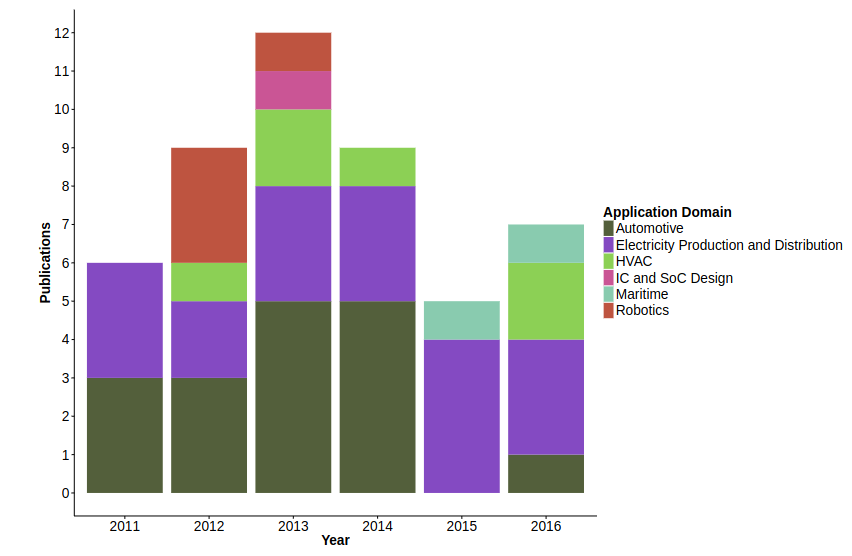
\includegraphics[width=0.7\linewidth]{Images/CoSimDifApps.png}
 	\caption{Research publications of co-simulation applications over five years\cite{gomes2017co}}
	 \label{fig_CoSimDifApps}
\end{figure}

One of the challenges when running a \gls{des} co-simulation is synchronization. As previously mentioned, there are different 
iterations of different abstraction levels, which can result in temporal misalignment. In other words, causality errors can happen due to a 
distinct time granularity. This problem is similar to the one faced when executing a parallel simulation, and the solutions applied to address 
them are remarkably consistent. 


\subsection{Gem5 and SystemC}

SystemC is being widely used in the industry and research hardware design space exploration \cite{menard2017system}. Nonetheless, there 
is a notable scarcity of precise, freely available, adaptable, and lifelike SystemC models for contemporary \glspl{cpu}. Christian Menard 
in \cite{menard2017system} developed an \gls{api} that allows full interoperability between the two simulators. 

In the paper, there are presented three possible scenarios for the co-simulation environment. The issue here is that achieving 
this co-simulation requires compiling Gem5 as a library and then using it in SystemC. This does not fully adhere to the previously mentioned 
co-simulation definition because the two simulators are not running simultaneously in separate processes. This limitation can lead to 
verification failures as direct inputs from other simulators to Gem5 are not possible.

% \begin{figure}[H]
% 	\centering
%  	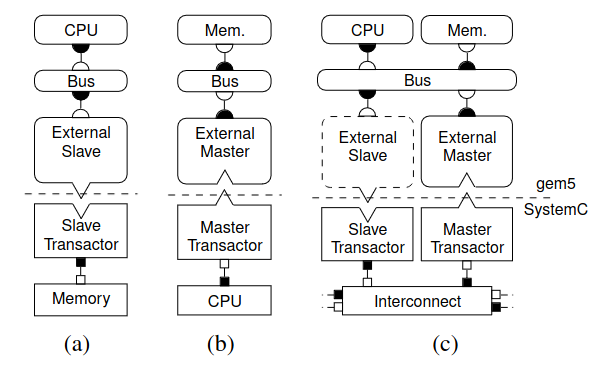
\includegraphics[width=0.7\linewidth]{Images/SystemCGem5_CoSim.png}
%  	\caption{SystemC and Gem5 interoperability \cite{menard2017system}}
% 	 \label{fig_SystemCGem5_CoSim}
% \end{figure}
